\documentclass[oneside,a4paper,13pt]{article}

\usepackage[utf8]{inputenc}
\usepackage[frenchb]{babel}
\usepackage{graphicx}
\usepackage{subcaption}
\usepackage{amsmath}
\usepackage{float}
\usepackage{geometry}
\usepackage{listings}
\usepackage{fancyhdr}
\lstset{
  language=bash,
  basicstyle=\ttfamily,
  showspaces=false,
  showtabs=false,
  showstringspaces=false
}
\geometry{hmargin=2.5cm,vmargin=1.5cm}
\captionsetup{compatibility=false}
\AtEndDocument{\label{lastpage}}

\usepackage{titlesec}
\usepackage{index}

\titleformat{\chapter}[display]
  {\Huge\bfseries}
  {}
  {0pt}
  {\thechapter.\ }
  
\titleformat{name=\chapter,numberless}[display]
  {\Huge\bfseries}
  {}
  {0pt}
  {}


\usepackage[latin1]{inputenc}
\usepackage[T1]{fontenc}
\usepackage[frenchb]{babel}

\pagestyle{fancy}
\fancyhf{}
\lhead{Rapport technique}
\rhead{Groupe 55}
\cfoot{\thepage/\pageref{lastpage}}
%\rfoot{Page \thepage}
%\lfoot{Rapport technique - Groupe 55}
  
\begin{document}

\title{ \textbf{Développement d'une application de reconnaissance manuscrite}\\ Rapport technique - Projet Codev}
\author{\textbf {Groupe 55} \\ Nicolas Servot\\Mahieu Pierronne\\Paul Michel\\Hugo Bouchez}
\date{\today}

\maketitle
\begin{figure}[H]
    \centering
    
\includegraphics[scale=0.7]{Images/Logo_IMT.png}
    \label{fig:neural_network}
\end{figure}

\newpage

\section*{Couverture}
Ce document correspond au rapport technique du projet Codev « Machina », projet réalisé et développé par le groupe 55. Le groupe était composé de quatre étudiants FISE 1A de IMT Atlantique : Nicolas Servot responsable backend et intégration, Hugo Bouchez responsable machine Learning, Paul Michel et Mathieu Pierronne responsables du Front End de la page web et du lien avec le serveur.\\
Ce rapport est à destination du comité de pilotage CODEV. Le projet a été encadré par Julien Mallet.  

\medbreak
Pour des raisons de simplicité chaque responsable s’est chargé de la rédaction de sa partie de développement web. Ainsi la partie Deep Learning a été écrite par Hugo Bouchez, la partie BackEnd par Nicolas Servot, la présentation du projet, la partie FrontEnd et la conclusion par Mathieu Pierronne. Paul Michel s’est quant à lui chargé de la relecture et de la correction de l’orthographe. 
\bigskip

\section*{Résumé}

Si l’écriture manuscrite est un excellent exercice cognitif qui stimule l'intelligence et les capacités cérébrales des élèves, elle est moins flexible que l’écriture numérique, qui peut être corrigé, modifié, et mise en forme en temps réel. Pour que les élèves de IMT Atlantique puissent à la fois bénéficier des avantages cognitifs et de mise en page respectivement des écritures manuscrite et numérique, nous avons décidé de mettre au point une application de reconnaissance manuscrite. 
\smallbreak
Un élève pourra prendre des notes sous forme papier, les numériser par l’intermédiaire de l’application pour pouvoir les modifier ensuite à sa guise et les archiver plus facilement. Cette application sera composée de trois parties : un algorithme de Deep learning de reconnaissance manuscrite, d’une interface web permettant à l’élève d’importer une image contenant des caractères manuscrits et d’un serveur faisant le lien entre ces deux éléments. 
\smallbreak
Le développement technique de ce projet se divise en trois grandes parties. Après avoir présenté les contraintes et fonctionnalités imposées par le client, nous présenterons la conception et la réalisation technique de l’algorithme de machine learning, de la partie Frontend et Backend. Cette partie inclut également les choix techniques réalisés et les difficultés rencontrées. Enfin, nous présenterons les résultats et la partie intégration de notre application. 
\medbreak

\textit{Rédateur} : Mathieu, \textit{Relecteur} : Nicolas

\textbf{Mots clés} : Machine Learning, développement web, Base de données



\section*{Abstract}
While handwriting is an excellent cognitive exercise that stimulates students' intelligence and brain capacity, it is less flexible than digital writing, which can be corrected, modified, and formatted in real time. In order for students at LMI Atlantic to benefit from the cognitive and layout advantages of handwritten and digital writing respectively, we decided to develop a handwriting recognition application. 
A student will be able to take notes in paper form, scan them through the application so that they can be edited and archived more easily. This application will be composed of three parts: a deep learning algorithm for handwritten recognition, a web interface allowing the student to import an image containing handwritten characters and a server linking these two elements. 
\smallbreak
The technical development of this project is divided into three main parts. After presenting the constraints and functionalities imposed by the customer, we will present the design and technical implementation of the machine learning algorithm, the frontend and backend part. This part also includes the technical choices made and the difficulties encountered. Finally, we will present the results and the integration part of our application. 


\newpage
\tableofcontents

\section{Introduction}
La reconnaissance d’écriture manuscrite est l’un des plus vieux problèmes qui ait été posé à l’intelligence artificielle, depuis son avènement dans les années 1950. Ce problème complexe d’IA met en jeu toutes les composantes de l’intelligence artificielle : pour comprendre et reconnaître une écriture manuscrite il faut visualiser une image, détecter le texte, suivre le tracé de l’écriture puis reconnaître les caractères, les mots et enfin les phrases. La reconnaissance d’écriture manuscrite est alors, au même que titre que la reconnaissance de la parole ou la traduction automatique, à la fois un terrain de jeu incontournable des nouveaux algorithmes d’apprentissage et un véritable défi scientifique et technique.\bigbreak
Dans un contexte d’explosion technologique, cette numérisation de documents manuscrits peut présenter de nombreux avantages, aussi bien pour usage pédagogique que professionnel. En effet, si de multiples études cognitives ont démontré l’importance de l’écriture manuscrite dans l’apprentissage et le développement intellectuel d’un enfant [1], l’écriture sur papier manque néanmoins de flexibilité : peu de modifications et corrections peuvent y être apportées. La reconnaissance d’écriture cursive permettrait alors de concilier les bienfaits de l’écriture manuscrite et de l’écriture numérique. Un travail pourrait être réalisé sous forme manuscrite, convertie ensuite en caractères typographiques pour enfin être traité, modifié, mise en forme, partagé et archivé comme on le souhaite. \bigbreak
Notre objectif dans ce projet est de développer une plateforme web permettant de convertir des documents manuscrits sous un format texte. Les utilisateurs de la plateforme pourront importer une photo contenant du texte manuscrit sur le serveur. Cette image sera analysée par un algorithme de reconnaissance, traitée puis renvoyée à l'utilisateur sous la forme d’un fichier texte \bigbreak
Ce rapport a pour objectif de donner un résumé des différents travaux faits durant le projet et de présenter les divers résultats obtenus. Dans un premier temps, nous aborderons le fonctionnement global de l’application. Ensuite, nous présenterons les différentes étapes de conception et de développement du Frontend, du Backend et de l’algorithme de Deep Learning. Enfin, dans une dernière partie, nous expliciterons la démarche d’intégration adoptée et présenterons les fonctionnalités validées durant ce projet.
\smallbreak\textit{Rédateur} : Mathieu, \textit{Relecteur} : Nicolas 
\bigskip


\section{Présentation du projet}

\subsection{Détail du besoin du client}
L’écriture manuscrite est un excellent exercice cognitif qui stimule les capacités cérébrales des élèves, en développant notamment leur mémoire, leur pensée et leur motricité [2].Il s’agit d’un exercice mental qui sollicite constamment le développement des connexions neuronales et contribue à l’autorégulation, à l’autodiscipline, à la volonté et à la persévérance. Les neurosciences ont montré que l’écriture à la main contribue à l’expansion du cerveau et stimule l’intelligence. De plus, lors de réunions, d’exposés ou des séances de formation, la prise de note manuscrite semble s’avérer plus efficace et plus productive que la prise de note numérique. La prise de note et l’écriture manuscrite semblent alors indispensables dans la formation et le développement intellectuel d’un étudiant. Cependant, malgré tous les bienfaits de l’écriture manuscrite, les documents papier sont problématiques puisqu’ils ne peuvent être modifiés, corrigés en temps réel et leur archivage et partage est bien plus compliqué. \medbreak
Le projet Machina est donc de concevoir une application permettant aux élèves de IMT Atlantique de convertir du texte manuscrit en caractères typographiques. Cette application permettrait aux étudiants de l’école de bénéficier à la fois des avantages de l’écriture manuscrite et de l'écriture numérique. Ils pourront prendre des notes sous forme papier, les numériser par l’intermédiaire de l’application pour les modifier ensuite  à leur guise et les archiver plus facilement.\medbreak
Une page d’accueil permettrait à l’élève d’importer une image contenant du texte cursif. Cette image serait ensuite traitée et analysée par le serveur puis convertie sous format texte. Le nouveau fichier texte pourra enfin être téléchargé sur la machine de l’utilisateur. \\
Cette partie recense les fonctionnalités, les contraintes et les critères de validation imposés par le client. 
\smallbreak\textit{Rédateur} : Mathieu, \textit{Relecteur} : Paul 

\subsubsection{Fonctionnalités requises}
Deux types de fonctionnalités devront être développées au sein de l'application web : des fonctionnalités client, qui seront les fonctionnalités essentielles au bon fonctionnement de l'application et des fonctionnalités administrateur, qui permettront de gérer l'accès des utilisateurs à l'appplication. \\
Tout d’abord, les fonctionnalités devant être développées d’un point de vue client sont : 

\begin{enumerate}
    \item Pouvoir importer une image sous format \emph{jpeg} ou \emph{png} contenant de l’écriture cursive. Cette image sera envoyée au serveur pour être traitée par l'algorithme de reconnaissance. 
    
    \item Pouvoir télécharger sous format texte la prédiction faite par l'algorithme. Ce texte pourra ensuite être modifié et archivé par l'utilisateur.
    
    \item Créer un compte avec son adresse mail IMT Atlantique, par le biais de la page d’authentification. Ce compte servira de clé d'authentification pour accéder aux diverses fonctionnalités de l'application. \\
    \textit{Seul les utilisateurs possédant un compte pourront accéder à l’application pour sécuriser son accès. La création du compte se fait en rentrant son adresse de l’IMT Atlantique, un nom d’utilisateur et un mot de passe.}
    
    \item Se connecter à l’application par le biais de la page d’authentification.\\
    \textit{La connection se fait en rentrant le nom d’utilisateur ou l’adresse mail associée, et le mot de passe adéquat. L’utilisateur arrive alors sur la page d’accueil, page permettant d'importer les images à traduire sous format texte.}
\end{enumerate}

\medbreak
Ensuite, les fonctionnalités devant être développées d'un point de vue administrateur, servant principalement à gérer la liste des utilisateurs ayant les droits d'accès à l'application, sont :  

\begin{enumerate}
    \item Se connecter à l’application par le biais de la page d’authentification.\\
    \textit{La connection est similaire à celle d’un client cependant l’administrateur arrive sur la page administrateur, qui lui permet d’effectuer les fonctionnalités suivantes.}
    
    \item Ajouter un utilisateur en entrant son nom d’utilisateur, son adresse mail de l’IMT Atlantique et son mot de passe.
    \textit Il y aura une section spécifique sur la page administrateur pour ce genre de requête.
    
    \item Retirer un utilisateur de la base données.
    \textit Il y aura une section spécifique sur la page administrateur pour ce genre de requête.
\end{enumerate}

\subsubsection {Contraintes de développement}

Lors du développement de l’application, certaines contraintes devront être respectées : 

\begin{enumerate}
    \item \textbf{Maintenabilité}\\
    Afin d’assurer la maintenabilité du site, il devra être développé en utilisant des technologies universelles comme le MEAN ou LAMP stack.
    L’algorithme de prédiction doit également être maintenable au possible. Dans une optique d’universalité, il sera développé en python et basé sur les bibliothèques sklearn et mlpy. 
    Enfin, il serait souhaitable d’appliquer une documentation systématique des pratiques de développement et détailler chacune des fonctionnalités mises au point pour faciliter une potentiel reprise du projet. 
    
    \item \textbf{Temps de traitement de la requête}\\
    Pour le temps de réponse du client, il serait souhaitable d’afficher la requête de l’utilisateur sous une seconde (le facteur décidant étant ici la quantité de donnée à traiter par l’algorithme de prédiction). 
Un certain dynamisme de site est également attendu : il devra être possible d’effectuer une recherche sans avoir à recharger entièrement la page.

    \item \textbf{Protocole de sécurité}\\
    L’application web ne pourra être accessible qu’à des membres du personnel et aux étudiants IMT Atlantique. Il faudra alors définir au préalable une base de données des personnes pouvant accéder à la plateforme et développer par la suite une page d’authentification à la plateforme. Les entrées de cette page d’authentification seront une adresse mail imt-atlantique et un mot de passe. S’il s’agit d’une première connexion, l'utilisateur devra cliquer sur un bouton “première connexion”. Il sera alors redirigé vers une seconde page où il devra entrer nom, prénom, adresse mail imt-atlantique et son mot de mot de passe. Si l’adresse mail sélectionnée n’appartient pas à notre base de données, son accès lui sera refusé. 
\end{enumerate}

\subsubsection{Critères de validation}
La reconnaissance manuscrite sera considérée comme fiable et valide si le coefficient de corrélation entre la texte numérisé et manuscrit est supérieur à 0,9, c’est-à-dire que plus de 9 lettres sur 10 du texte manuscrit concordent avec la proposition faite par l’algorithme de reconnaissance. 
\smallbreak\textit{Rédateur} : Mathieu, \textit{Relecteur} : Paul


\subsection{Description générale de l'application}
L’application sera composée de trois parties principales : 

\begin{enumerate}
    \item Un algorithme de Deep Learning qui aura pour rôle d’identifier l’écriture cursive présente sur l’image importée par l’utilisateur, pour la convertir ensuite en un format texte modifiable. Cette reconnaissance d’écriture manuscrite se fera en deux temps : 
    \begin{enumerate}
        \item Dans un premier temps, une prédiction est effectuée sur l'ensemble des mots par l'algorithme de deep learning constitué d'une succession de couche neuronal préalablement entraînée à la détection de texte.
        \item Puis, dans un second temps, le résultat de la prédiction est comparé avec un dictionnaire de mot employés dans le langage utilisé. L'algorithme renverra, après comparaison, le mot le plus probable contenu dans le dictionnaire à l'utilisateur.   
    \end{enumerate}
    
    \item Une application web qui correspondra à l’interface Homme/Machine. Cette application sera composée  de trois pages principales :
    \begin{enumerate}
        \item Une page “login” permettant aux utilisateurs de se connecter à l’application via une adresse mail imt-atlantique et un mot de passe. 
        \item Une page “registrer” permettant aux nouveaux utilisateurs de se créer un compte. Une création de compte ne sera possible qui si l’adresse mail saisie fait partie de la base des données des membres du personnel et étudiants IMT Atlantique.
        \item Une page “administrateur” permettant au gestionnaire de la page de gérer les nouveaux membres du site. 
        \item Une page “accueil”, qui sera la page principale et qui permettra à l’utilisateur d’importer la photo qu’il souhaite traiter et de télécharger ensuite sous format texte la numérisation faite par l’algorithme de reconnaissance. 
    \end{enumerate}
    
    \item Un serveur qui aura pour rôle de faire le lien entre l’algorithme d’apprentissage et la plateforme web décrite ci-dessus. C’est dans ce serveur que seront stockées toutes les informations des utilisateurs et les statistiques de l'algorithme de reconnaissance manuscrite. 
\end{enumerate}

\bigbreak
Maintenant que nous avons présenté l'architecture globale de l'application nous allons décrire plus en détail les partie de conception et de réalisation de l'algorithme de reconaissance, du Frontend et du Backend. 
\smallbreak\textit{Rédateur} : Mathieu, \textit{Relecteur} : Paul




\section{Développement de l'algorithme de reconnaissance manuscrite}

\subsection{Introduction brève à l'apprentissage profond}
\subsubsection{Architecture d'un réseau de neurone}
L'apprentissage profond ou Deep Learning appartient à la classe des méthodes d'apprentissage supervisées (ML) basée sur des réseaux de neurones artificiels. Le modèle de Deep learning (DL) est très utile dans les domaines de la reconnaissance auditive, la reconnaissance d'images, la traduction, etc. Les réseaux de neurones artificiels de DL ont été inspiré par l'architecture du système biologique en tant que réseau neuronal humain. \\
Un réseau de neurones est essentiellement composé de couches, elles-mêmes composées de neurones. La première couche est appelée \emph {Input Layer}, la dernière couche est la \emph {Output Layer} et toutes les couches intermédiaires sont les \emph {Hidden Layer}. Un réseau neuronal composé de plusieurs couches est appelé réseau neuronal profond. L'idée est de relier la sortie de chaque neurone de la couche N à l'entrée de la couche (N + 1). Après cela, l'entraînement du modèle, qui consiste littérallement à le "nourrir" en lui demandant de traiter des données d'entrées et en comparant ses prédictions avec les résultats attendus, ne fait que changer le poids alloué à chaque lien.[3]\\ \\
Pour comprendre précisément la structure d'un réseau de neurones, penchons nous à présent sur le fonctionnement d'un neurone classique.
\begin{figure}[H]
    \centering
    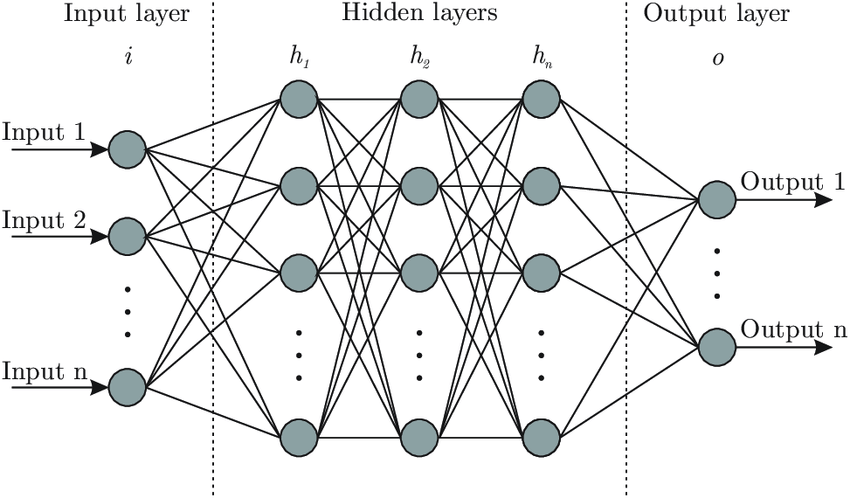
\includegraphics[scale=0.3]{Images/Artificial-neural-network-architecture-ANN-i-h-1-h-2-h-n-o.png}
    \caption{Illustration d'un réseau de neurone profond standard}
    \label{fig:neural_network}
\end{figure}
\subsubsection{Description du fonctionnement classique d'un neurone}
Pour illustrer le fonctionnement d'un réseau neuronal, prenons l'exemple d'une seule couche composée d'un unique neurone.
\begin{figure}[H]
    \centering
    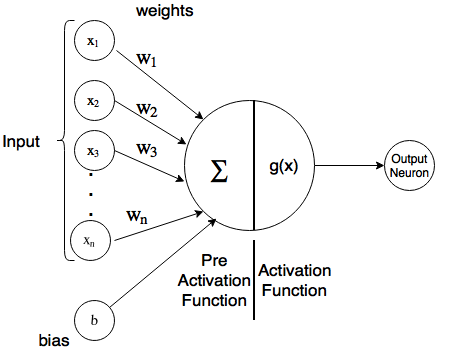
\includegraphics[scale=0.5]{Images/neron.png}
    \caption{Neurone artificiel}
    \label{fig:neuron}
\end{figure}
Un neurone classique effectue deux étapes lors de son activation. La première étape est le calcul de la \emph {fonction de Pré-activation}[4]
\begin{equation}
Z = \sum_{i \in I} x_{i}w_{i} + b
\end{equation}
On retrouve Z la valeur de la pré-activation, $w_{i}$ les poids associées à chaque inputs : $x_{i}$, enfin b, le \emph{bias} est un paramètre de linéarité de l'équation.\\
La seconde opération est l'\emph {Activation} du neurone. Elle représente la notion de "potentiel d'activation", seuil de stimulation qui une fois atteint entraîne une réponse du neurone. Pour un certain seuil, le neurone déclenche un 1 si le seuil est franchi, sinon un 0. Enfin, l'\emph {Output} est la valeur de la fonction d'activation:
\begin{equation}
Y = g(Z)
\end{equation}
La fonction \emph{Rectifier Linear Units} (ReLU) est la fonction d'activation la plus commune. D'autres fonction d'activation sont présentées en Annexes.
\begin{align*}
ReLU : Y = max(0,Z)
\end{align*}
Dans un réseau de neurones à plusieurs couches, il convient de que les inputs des neurones de la couche N soient les outputs des neurones de la couche (N - 1), l'existence d'un lien revient à dire que les neurones sont "connectés".\\ \\
Nous venons donc de découvrir la structure d'un réseau neuronal classique et le fonctionnement d'un neurone. Quelles sont à présent les opérations qui permettent de rendre de tels modèles performants ?
\smallbreak\textit{Rédateur} : Hugo, \textit{Relecteur} : Paul
\subsection{Entraînement du modèle}
Une fois le réseau neuronal définie, nous pouvons commencer la partie d'apprentissage avec l'entraînement du modèle. Dans ce réseau neuronal, un poids est affecté à chaque neurone. Ce poids permet de pondérer l'importance d'une certaine output par rapport aux autres. La valeur initiale de ces poids est attribuée aléatoirement lors de l'initialisation du modèle. L'étape d'apprentissage vise à modifier ces valeurs afin de créer un modèle efficace qui correspond au mieux à la réalité.\\
Pour cette étape d'apprentissage, nous devons définir quelques grandeurs mathématiques importantes. 
\subsubsection{La fonction coût, critère d'évaluation}
La fonction de coût, essentielle en apprentissage profond t est définie par : 
\begin{equation}
    E(Y) = \frac{1}{2}(Y - T)^{2}
\end{equation}
Avec T la cible à atteindre et Y la sortie du neurone.La fonction de coût représente une valeur quantitative de l'erreur, si la valeur du coût est faible alors l'erreur est faible et inversement. L'objectif de l'algorithme est de minimiser la valeur de E, de manière à ce que la valeur obtenue en sortie se rapproche le plus à la valeur attendue et souhaitée.\\ \\
Nous allons à présent examiner les méthodes pour diminuer ce coût.
\subsubsection{La descente de gradient et les méthodes d'optimisation}
La descente de gradient est un algorithme d'optimisation qui réduit la fonction de coût en actualisant les différents poids affectés à chaque neurones.
\begin{equation}
    {W_{k+1}} = W_{k} - \alpha\nabla(E)
\end{equation}
Avec :
\begin{align*}
W^{k} = [w_{0}^{k},w_{1}^{k},...,w_{i}^{k},...,w_{n}^{k}]^{T}\\ \\
\nabla(E) = [\frac{\partial E}{\partial w_{0}},...,\frac{\partial E}{\partial w_{i}},...,\frac{\partial E}{\partial w_{n}}]\\ \\
\alpha : \emph{taux d'apprentissage}\\
\end{align*}
La séquence $W_{k}$ correspond à la position actuelle, le taux d'apprentissage $\alpha$ impacte la vitesse d'apprentissage de l'algorithme, le gradient de la fonction de coût représente la direction de l'augmentation la plus rapide.
La séquence $W_{k}$ doit converger vers un minimum local si les paramètres ont été correctement sélectionnés.\\
Il y a beaucoup d'optimiseurs mais il ne serait pas nécessaire de les présenter dans cette section.
Dans le projet, l'optimiseur RMSprop sera utilisé, il n'y a approximativement aucune différence notable entre les deux optimiseurs, sauf que le RMSprop aide l'algorithme à converger plus précisément (il se concentre sur la bonne direction), en conséquence, le taux d'apprentissage peut-être plus élevé et le modèle converger plus rapidement.
\begin{figure}[H]
    \centering
    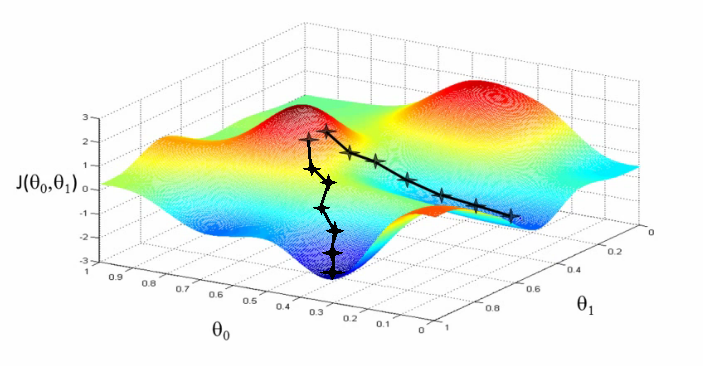
\includegraphics[scale=0.5]{Images/gradient_descent.png}
    \caption{Illustration de la descente de gradient}
    \label{fig:gradient_descent}
\end{figure}
\smallbreak\textit{Rédateur} : Hugo, \textit{Relecteur} : Paul

\subsection{Choix de la base de donnée}


La partie apprentissage définie précédemment doit reposer sur une base de données importante. C'est cette base de données qui va permettre à l'algorithme de s'entraîner pour être capable ensuite de reconnaître les caractères manuscrits de manière autonome. Le choix de cette base de donnée est déterminant sur les performances du modèle. Dans le domaine de la reconnaissance de texte manuscrit mais plus généralement en reconnaissance d'image, une base de donnée contenant des images trop spécifiques ou au contraire trop général peuvent diminuer la qualité des prédictions.\\
Le phénomène d'\textbf{Overfitting} ou \textbf{Surapprentissage} est un bon exemple concret permettant de comprendre pourquoi il est nécessaire de porter une attention toute particulière au contenu de la base de donnée.\\
Prenons un algorithme de reconnaissance d'image capable de déterminer si un cadre contient un chien ou n'en contient pas, Un modèle correctement construit s'appliquera alors à reconnaitre des motifs précis (oreilles, museau, pattes). Admettons à présent que toutes les photos de chien sélectionnées pour constituer la base de donnée ait été prise dans un salon avec un animal en position assise. Il est alors fort probable que l'algorithme ne soit pas en mesure de reconnaître un chien dans un jardin ou en train de courir. Ce phénomène est appelé Overfitting et intervient donc lorsque l'algorithme apprend des structures qui ne sont pas liées au problème. Enfin le modèle peut "sur-apprendre" d'autres manières encore, notamment si le modèle choisi est inadapté (linéaire, non-linéaire) ou si le temps d'apprentissage est trop long ce qui peut introduire de l'apprentissage "par coeur".
\subsubsection{Le problème de la langue}
Le premier choix qui doit être réalisé est le choix de la langue du texte à prédire. En effet, un modèle de reconnaissance manuscrite ne se concentre pas seulement sur la reconnaissance de motifs, en d'autres termes, la méthode pour prédire un mot n'est pas celle qui consisterait à prédire chacune de ses lettres. Des facteurs comme la fréquences d'apparition des lettres ou certaines combinaisons de caractères peuvent influer sur la prédiction. Ainsi un algorithme de reconnaissance manuscrite ne sera pas aussi performant sur un texte qui n'a pas été écrit dans la langue avec laquelle il a été entraîné.
\subsubsection{L'importance du décodeur}
Un "décodeur" est un algorithme qui compare un mot donné à un ensemble de mot compris dans un dictionnaire pour en extraire celui avec le plus de similarité. Certaines méthodes utilisées peuvent se rapprocher de celles employées en cryptographie. Ramené à la reconnaissance manuscrite, un décodeur permet donc de renvoyer des mots qui appartiennent à la langue du modèle.
\bigbreak
Le choix de la base de données est donc primordial. Pour que l'algorithme de reconnaissance manuscrite fonctionne correctement, il faut une base de données fournie et diversifiée pour éviter le problème d'\textit{Overfitting} et il faut choisir convenablement le décodeur et la langue d'entraînement. Ensuite, pour que cette base de données soit analysée correctement par l'algorithme de reconnaissance, il est nécessaire de la traiter et de la simplifier en amont. 

\smallbreak\textit{Rédateur} : Hugo, \textit{Relecteur} : Paul

\subsection{Traitement de la base de donnée}

\subsubsection{Les fonctions de seuil}
Une photo brute est généralement très difficile à comprendre par un algorithme de reconnaissance : il y a plusieurs couleurs avec des nuances plus ou moins marquées. Pour simplifier l'apprentissage de l'algorithme de reconnaissance, il est nécessaire de convertir une image colorée en une image en noir et blanc, avec l'écriture en pixels noirs et le fond en pixels blancs. \\
Pour appliquer ce traitement aux images de la base de données, on utilise une fonction de seuil. Cette fonction de seuil est une fonction booléenne qui détermine si oui ou non une valeur a dépassé un certain seuil. Dans le domaine du traitement de données, elle est utilisée pour convertir les pixels gris (mis à l'échelle entre 0 pour les pixels noirs et 255 pour les pixels blancs) en pixels binaires (Vrai et Faux) représentant le noir et blanc. Dans le cadre du projet, l'objectif était de transformer l'arrière-plan en pixels blancs et le texte manuscrit en pixels noirs. En supposant que le texte est écrit sur une feuille vierge, dans la plupart des cas, la valeur des pixels du texte sera la plus faible. La valeur 100 qui détermine si un pixel est vrai ou faux a été choisie arbitrairement sur la base de l'expérience.
\begin{figure}[H]

\begin{subfigure}{0.5\textwidth}
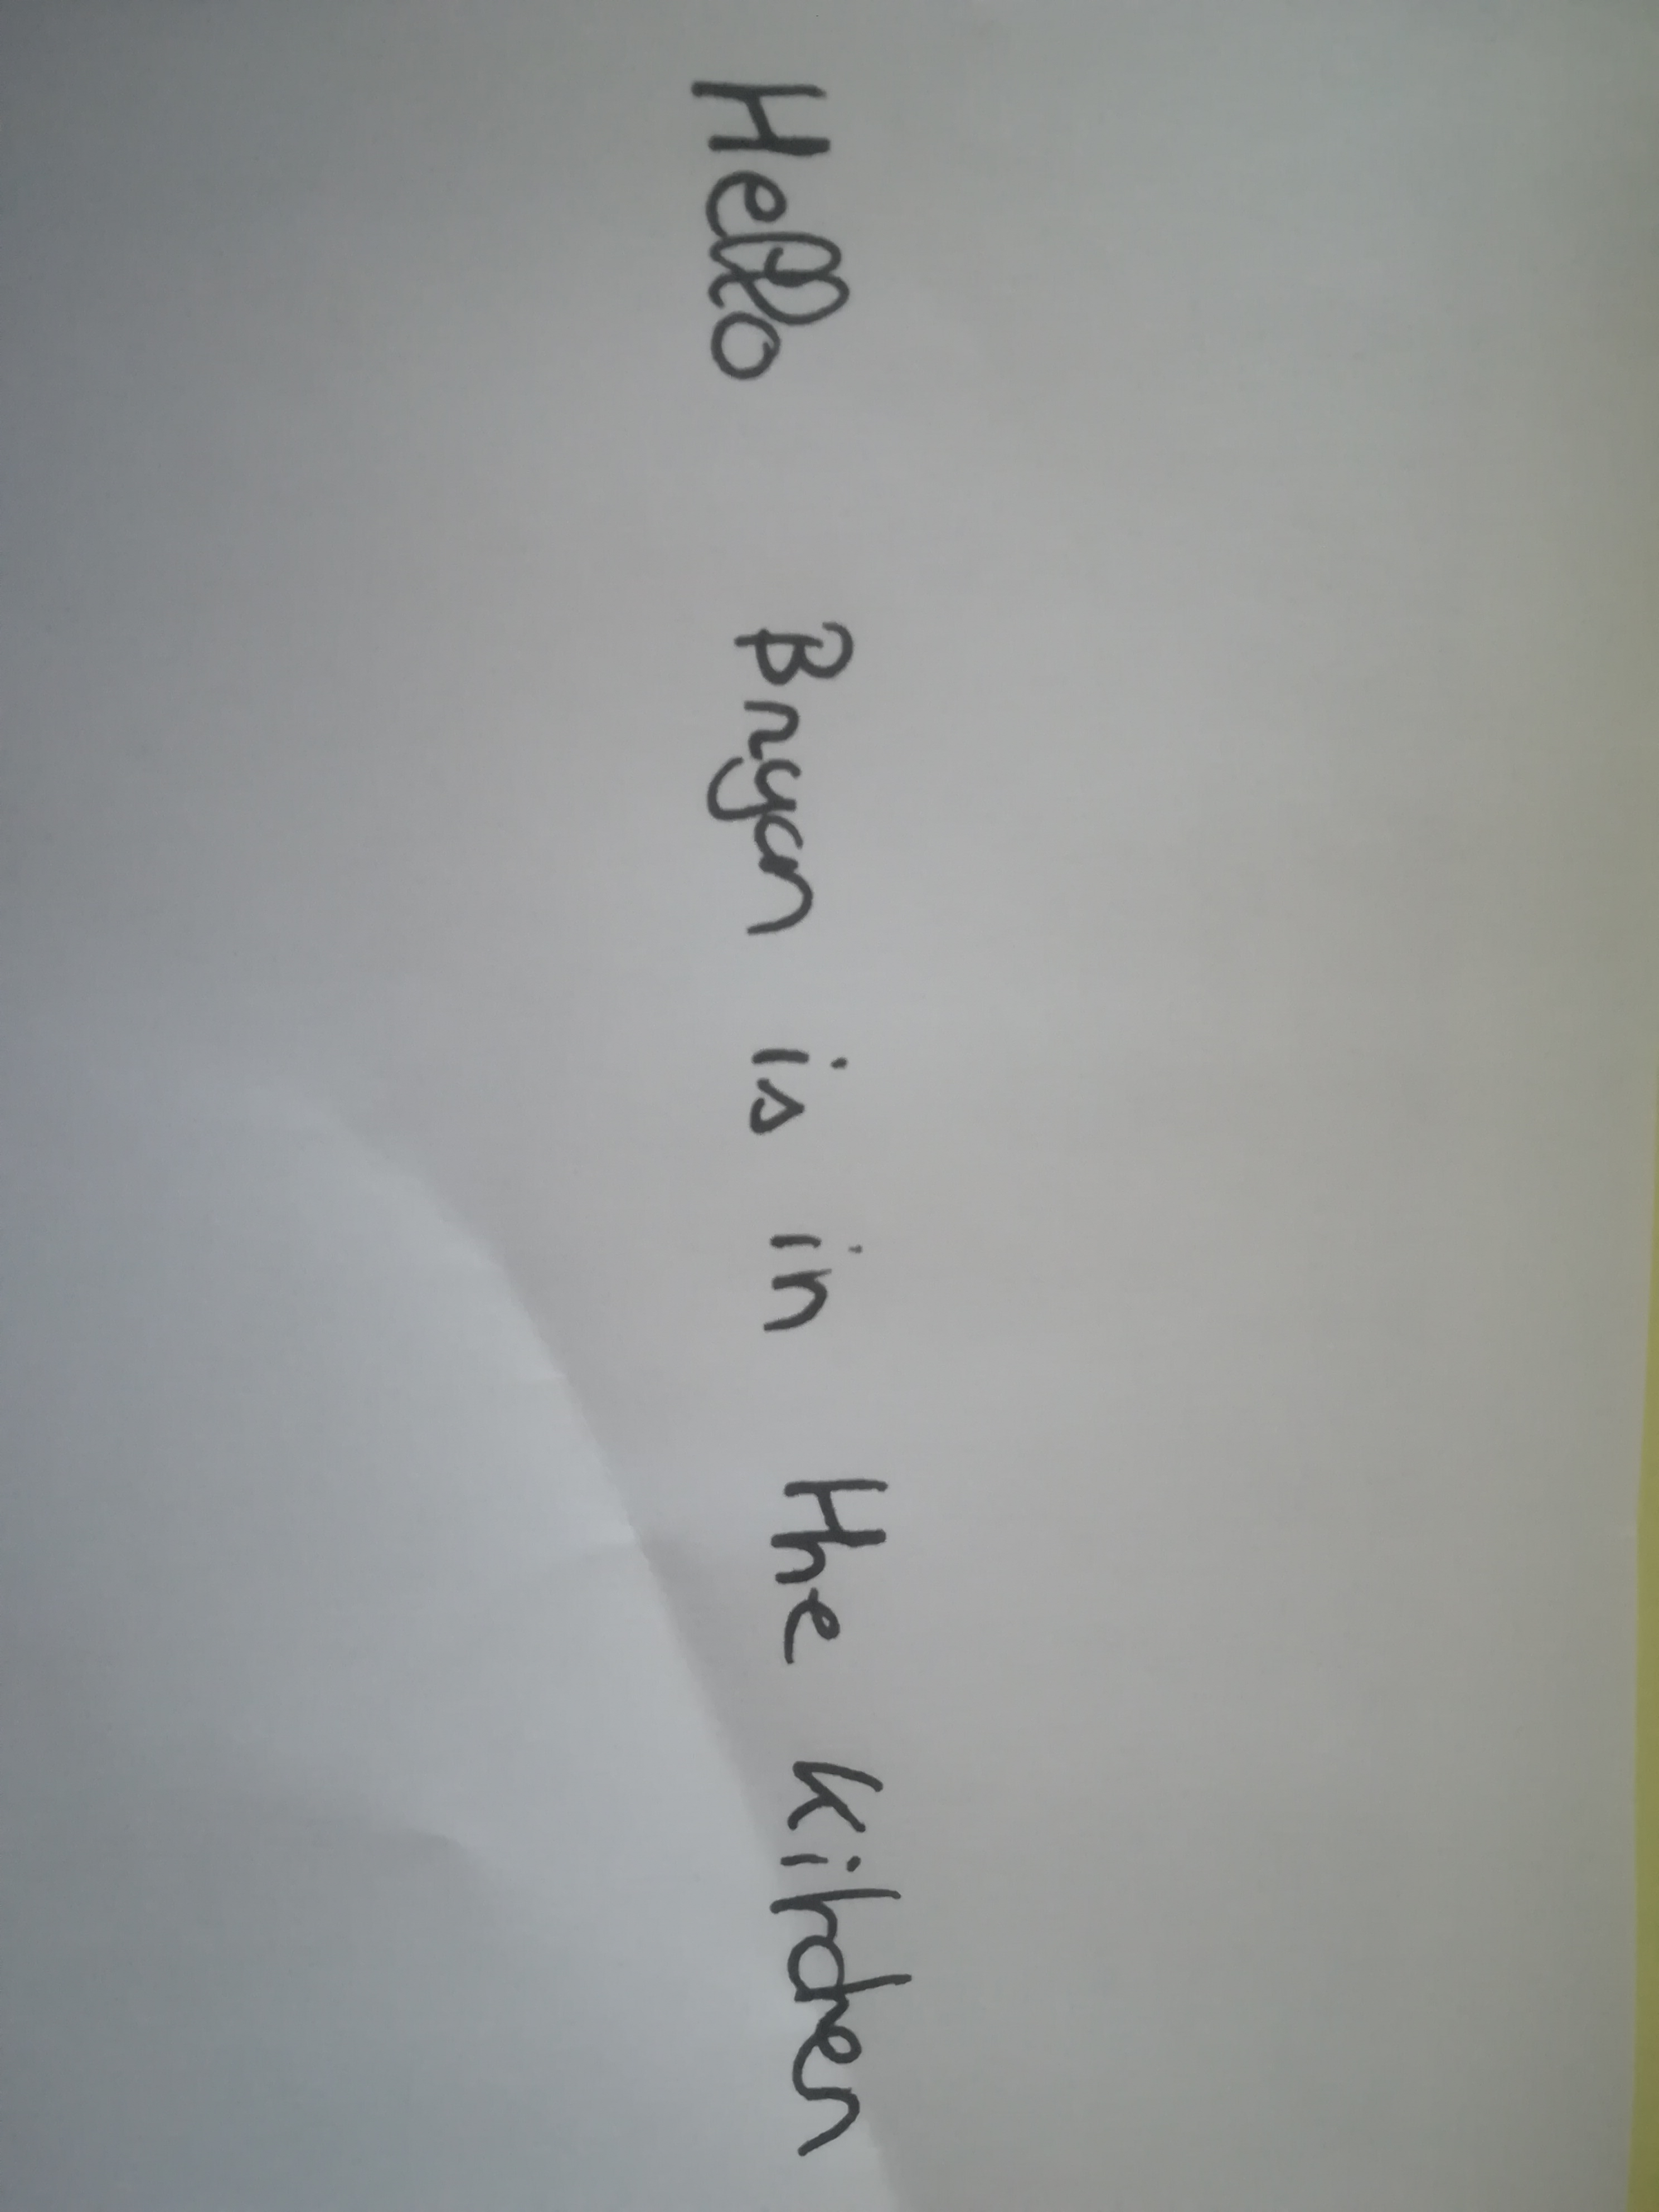
\includegraphics[width=0.9\linewidth,height=5cm]{Images/testCodev.jpg} 
\caption{Image avant application de la fonction seuil}
\label{fig:subim1}
\end{subfigure}
\begin{subfigure}{0.5\textwidth}
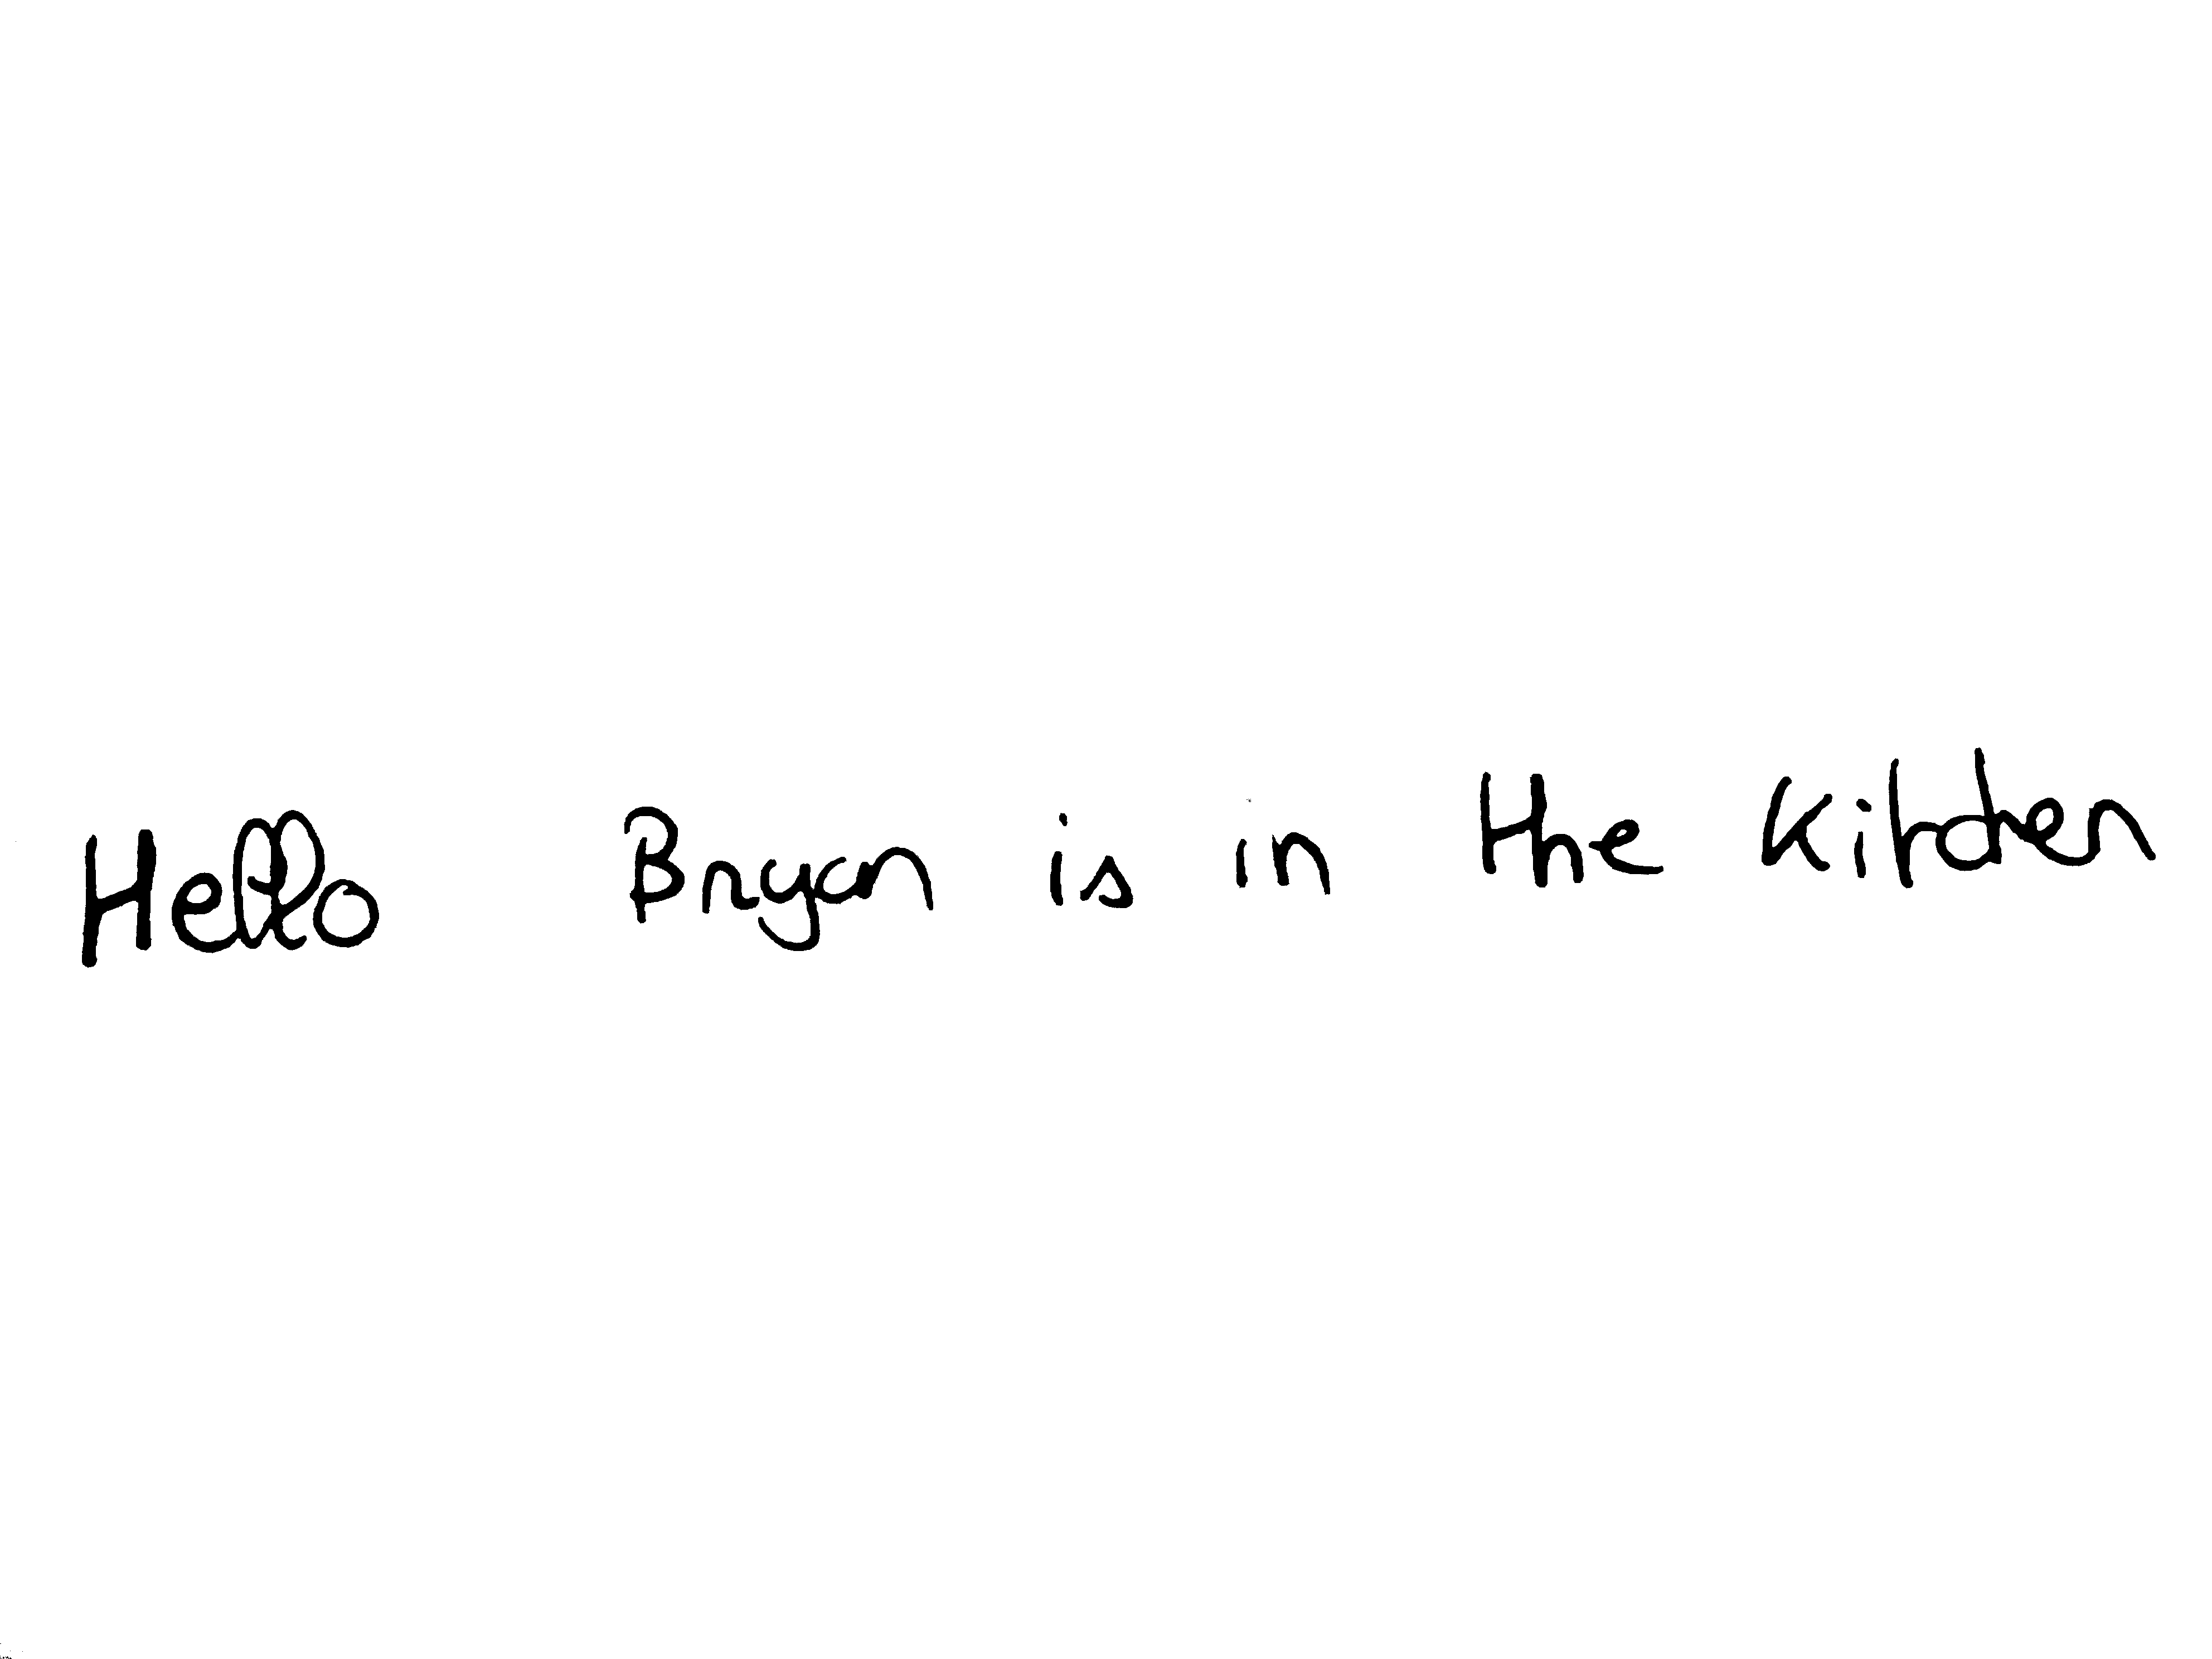
\includegraphics[width=0.9\linewidth, height=5cm]{Images/th_img.png}
\caption{Image après application de la fonction seuil}
\label{fig:subim2}
\end{subfigure}

\caption{Effet de la fonction de seuil}
\label{fig:image1}
\end{figure}


\subsubsection{Extraction des "Bounding Boxes"}
Une fois que l'ensemble de l'arrière plan a été converti en pixels blancs et le texte en pixels noirs, la phrase doit être fractionnée et divisée sous forme de mots. Cette étape est appelée "Extraction des Bounding Boxes". 
En partant d'une image A donnée, composée de mots et de bruits de fond, le script devra renvoyer les coordonnées (position X, position Y, largeur, hauteur) de chaque mot du fichier. \\
Le moyen le plus pratique pour obtenir ces coordonnées semble être Pytesseract, un package python basé sur une API Google open source, Tesseract. Ce package est vraiment utile dans le domaine de la reconnaissance optique de caractères, mais tout à fait inapproprié dans le domaine de la reconnaissance manuscrite.
\begin{figure}[H]
\centering
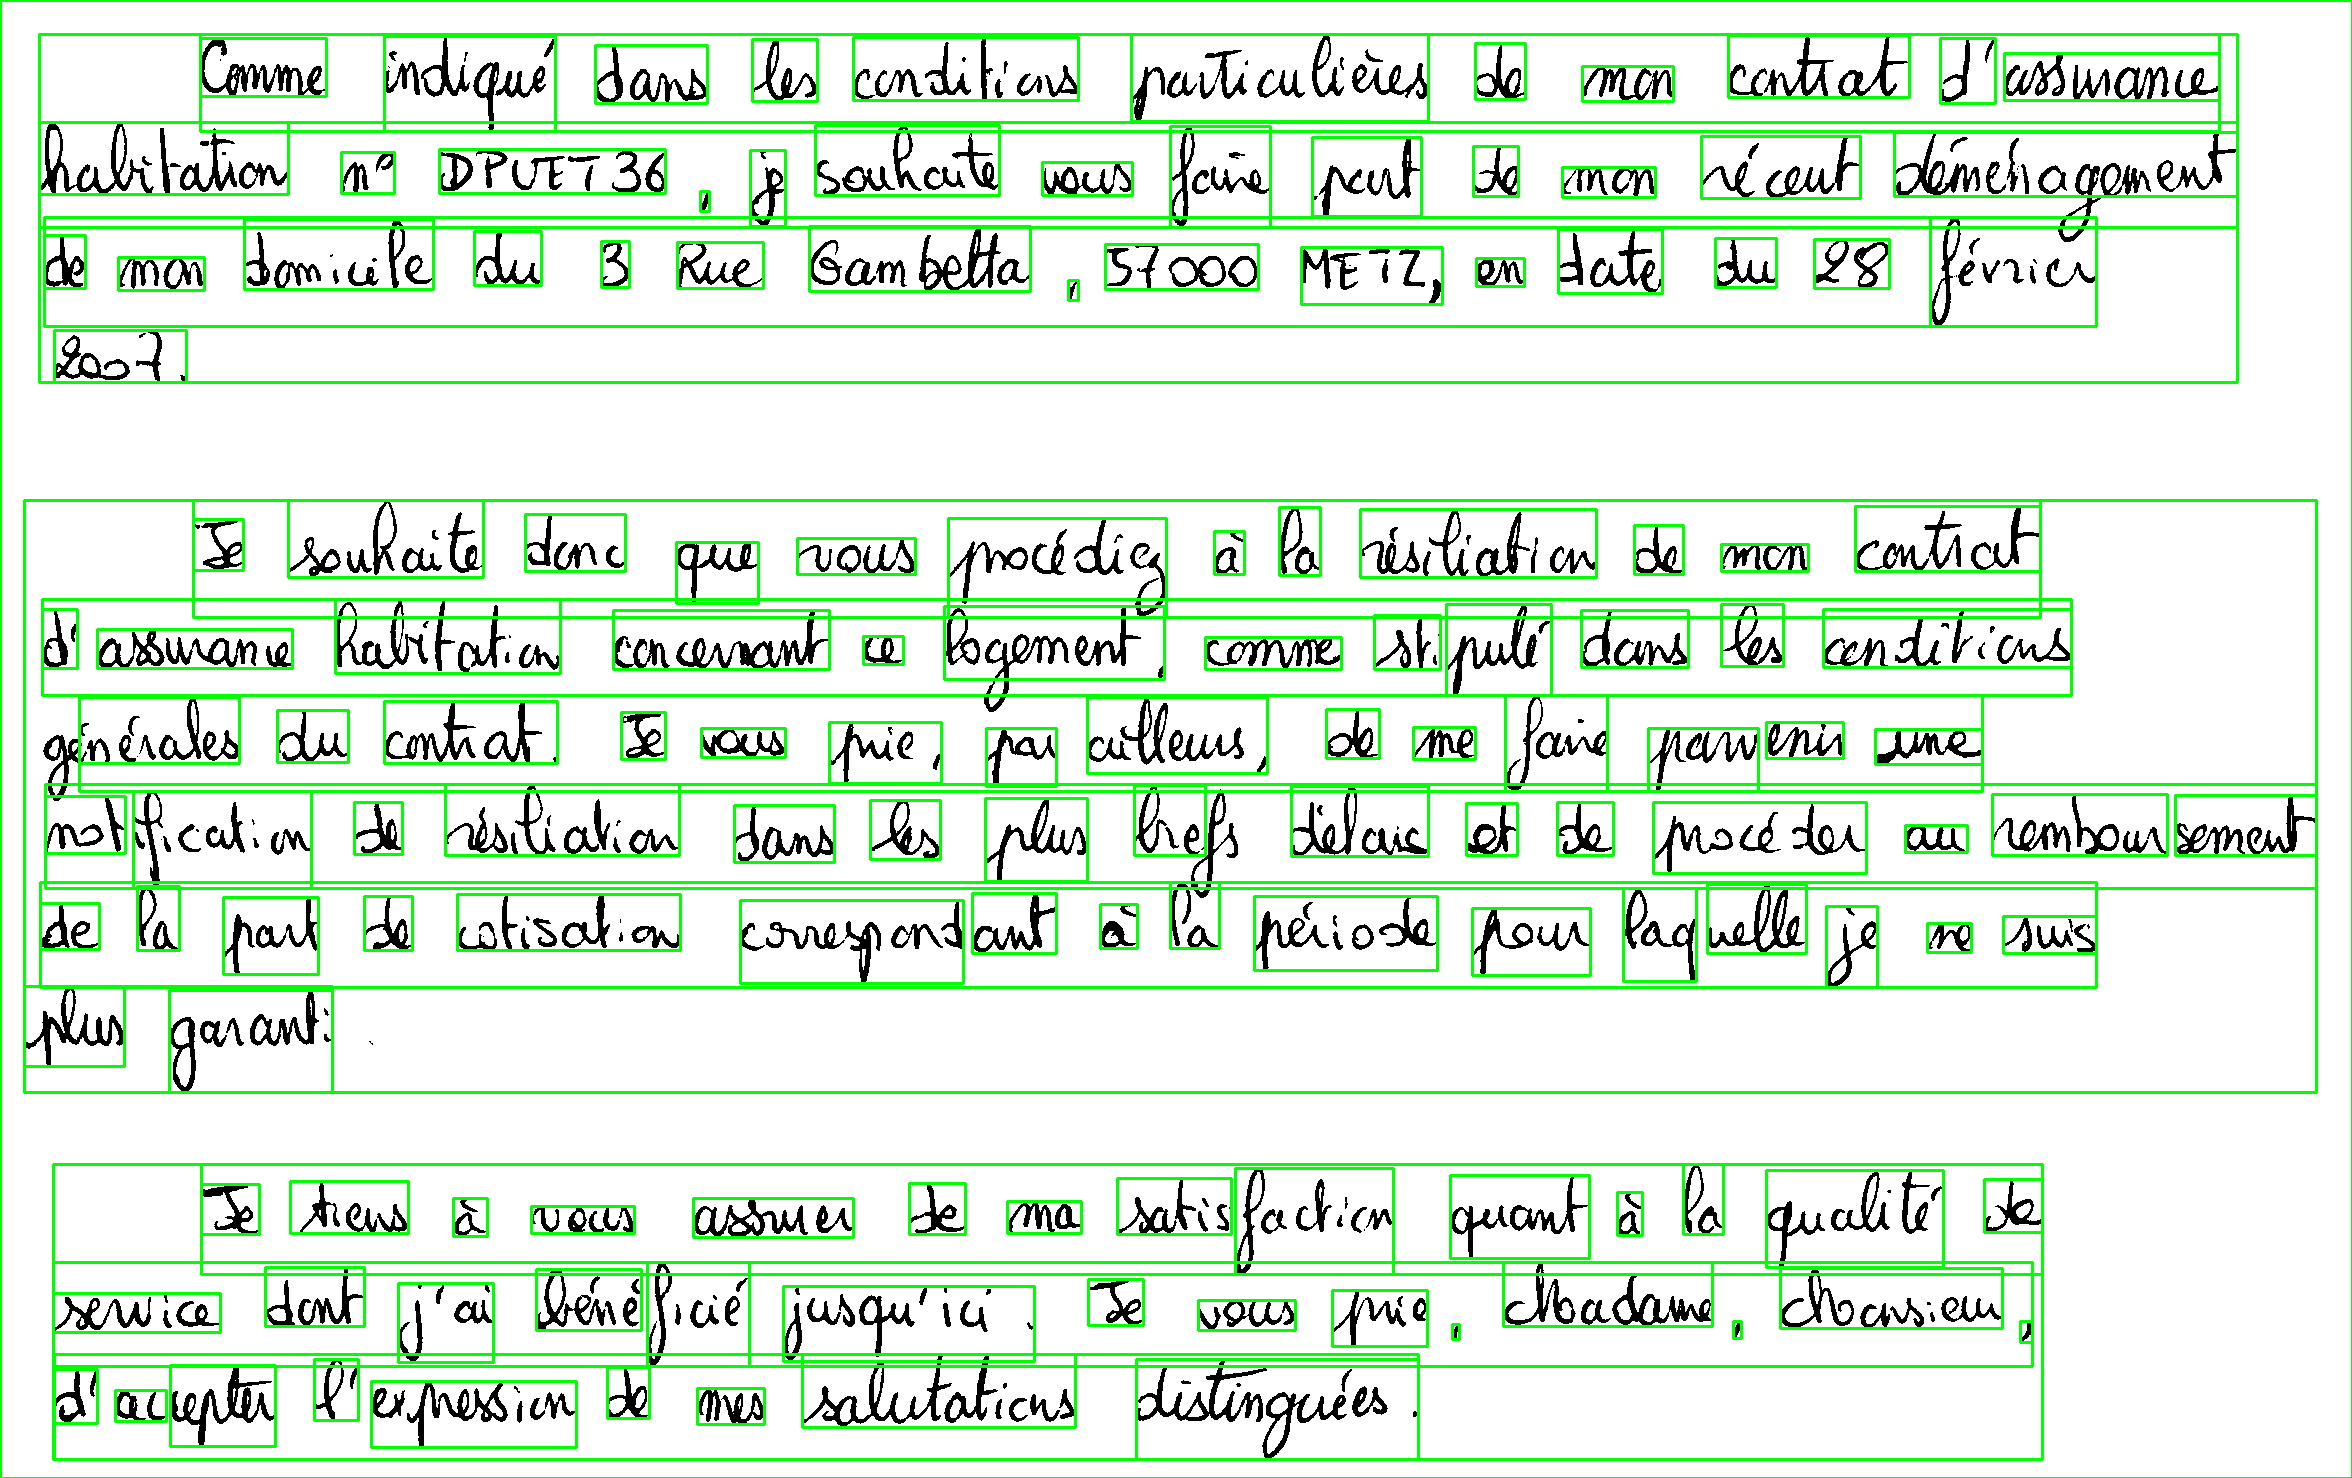
\includegraphics[width=0.7\textwidth]{Images/copy.png} 
\caption{Application de PyTesseract}
\end{figure}
\subsubsection{Normalisation des données}
Cette section vise plus à introduire la notion de normalisation des données et à décrire les méthodes employées au cours du projet que de présenter une liste exhaustive des méthodes de normalisation. \\ \\
Selon Wikipedia, la normalisation de la base de données "est le processus de structuration d'une base de données relationnelle selon une série de formes dites normales afin de réduire la redondance des données et d'améliorer l'intégrité des données". Pour illustrer cette définition, voici un petit exemple pour comprendre la notion de normalisation.
On considère un tableau de pixels RGB composé de triplets (R, G, B), où R, G et B représentent des nombres entiers compris entre 0 et 255, correspondant aux caractéristiques d'entrée de notre exemple. En entraînant le réseau de neurones avec cet ensemble de données, le poids des pixels blancs (255, 255, 255) risque de devenir supérieur au poids des pixels noirs (0, 0, 0). Il est alors nécessaire de normaliser les caractéristiques d'entrées pour éviter de rencontrer ce problème. \\ \\

La méthode de normalisation utilisé fût l'application d'une fonction de seuil pour convertir les données grises en pixels binaires.
Après cela, la dernière opération a été de redimensionner l'image pour obtenir un tableau 2D avec une taille de (128,32).

\bigbreak
Nous avons ainsi vu dans cette partie les grandes lignes de conception et de réalisation de l'algorithme de Deep Learning. Cet algorithme de reconnaissance est un réseau neuronale qui traite l'image (la convertie en noir et blanc, la fractionne en mots et normalise l'image), puis qui tente de deviner, à l'aide d'un entraînement au préalable et d'un dictionnaire de la langue étudiée, les mots présents dans le texte manuscrit. \\
Nous allons maintenant présenter le développement web : les choix de conceptions réalisés et les difficultés de développement rencontrées. 
\smallbreak\textit{Rédateur} : Hugo, \textit{Relecteur} : Paul


\section{Développement Frontend}

La partie Frontend correspond au design et au développement de l’interface web. Cette partie de développement agence et structure les éléments du site que l’on voit à l’écran et avec lesquels on peut interagir. Le développement Frontend facilite la vie de l’utilisateur : elle fait le lien entre le serveur, l’algorithme de reconnaissance et l’internaute, et améliore ainsi l’expérience de l’utilisateur. 
\smallbreak
Dans cette partie nous aborderons le travail de développement web effectué, les choix techniques réalisés ainsi que les solutions apportées aux différents problèmes rencontrés. 


\subsection{Détail du travail réalisé}
Pour avoir une idée plus précise du travail réalisé tout au long de ce projet, en ce qui concerne le développement de l’interface web, voici un diagramme de Gantt qui récapitule le déroulé des missions réalisées. Ce diagramme a été mis à jour tout au long du stage afin d’avoir un aperçu du travail réalisé mais aussi pour que nous puissions nous organiser pour finir le projet dans les meilleurs délais. 

\begin{center}
    \begin{figure}[H]
        \centering
        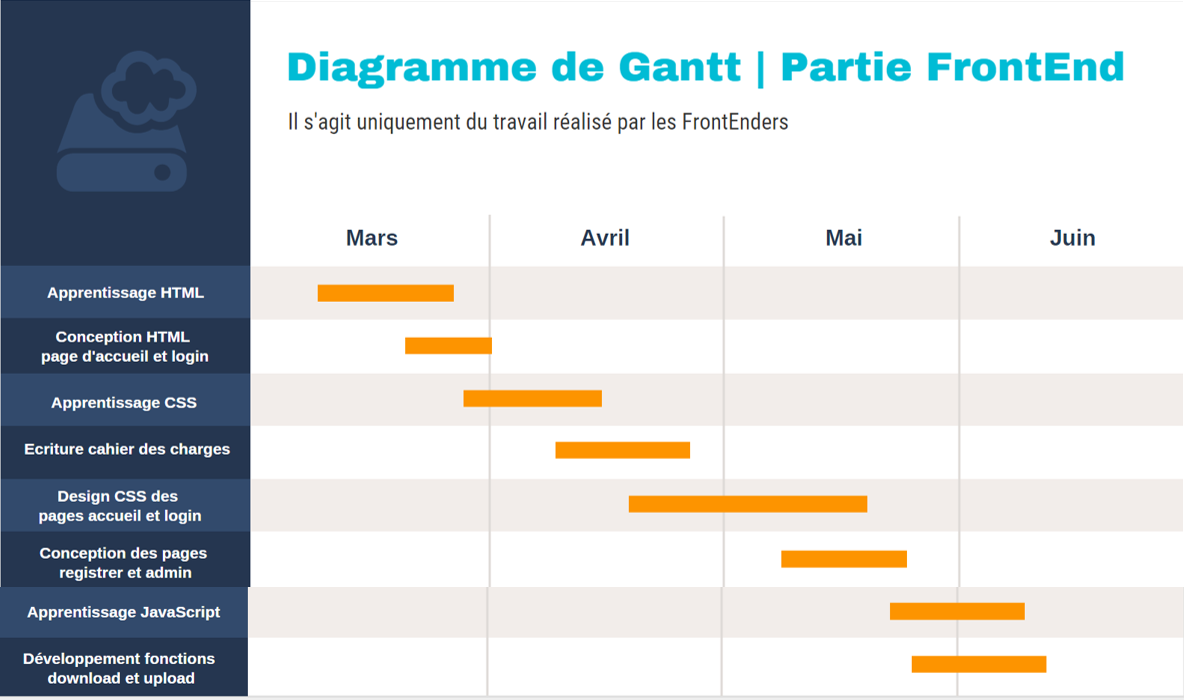
\includegraphics[scale=0.7]{Images/diagrammeGantt.png}
        \label{fig:neural_network}
        \caption{Diagramme de Gantt, partie Frontend}
    \end{figure}
\end{center}

\smallbreak\textit{Rédateur} : Mathieu, \textit{Relecteur} : Nicolas
\subsection{Choix techniques réalisés et description des langages}

Le langage de programmation utilisé va beaucoup influer sur le projet et la manière dont celui-ci sera développé, en fonction des avantages et des inconvénients du langage. Pour éviter de devoir changer de langage en cours de projet, ce qui constituerait une perte de temps considérable, il est essentiel de bien choisir le langage de programmation au préalable.  De plus, un langage optimisé et facile à apprendre permettra d’avoir une meilleure optimisation de la charge du CPU, ce qui aura pour conséquence de préserver le matériel et de faciliter la maintenance. Pour choisir un langage de programmation adéquat, il convient de comparer les langages disponibles entre eux. 
\smallbreak
Deux principales options de développement se sont imposées à nous :  une application mobile (développement natif) ou concevoir une application web.


\subsubsection{Application mobile : inconvénients des applications hybrides et natives}
Les étudiants étant plus amenés à utiliser cette application sur mobile, en prenant une rapide photo de leurs notes après un cours pour la convertir ensuite sous format texte, l’application mobile semblait plus adapté. 
Cependant, le développement d’une application mobile, que ce soit une application hybride ou native est moins intéressante d’un point de vue formatif et pédagogique.[11]
\bigbreak

\textbf{Applications hybrides}
\newline
\
Tout d’abord, pour le développement d’une application hybride, nous avions le choix entre les frameworks \textit{React Native} et \textit{Flutter} 
\begin{itemize}
    \item \textit{React Native} est un framework open source utilisant le langage Javascript. Si ce langage est très utilisé pour le développement de modules, il est très rare qu’il soit utilisé pour la conception entière d’une application. De plus, le framework \textit{React Native} ne prend pas en charge toutes les API natives. Cela aurait pu être problématique lors de l’intégration du système ou lors du partage de nos codes sur GitHub. 
    \smallbreak
    \item \textit{Flutter} quant à lui un framework créé par Google utilisant le langage Dart. Dart étant un langage peu universel mise au point récemment par Google pour remplacer Javascript, nous n’avons pas poursuivi cette piste. 
\end{itemize}
\smallbreak
Ces deux langages hybrides sont donc peu formateurs et peu intéressant pour un usage pédagogique. En plus de cela, les applications hybrides ne s’adaptent pas toujours bien aux systèmes d’exploitation IOS ou Android. Nous avons alors décidé de mettre cette solution de côté. 

\bigbreak 
\textbf{Applications natives}
\newline
\
On retrouve ce même problème pour les applications natives. En effet, nous aurions pu développer une application IOS avec le langage de programmation objet \textit{Swift}, ou \textit{Objective-C} ou développer une application Android en Kotlin ou C++. Cependant, ces langages de programmation objet sont,  pour la plupart, spécifiques à un serveur et peu universels. De plus, une telle application nous aurait contraint à un double développement pour permettre à tous les élèves, aussi bien ceux ayant un Iphone que ceux avec un smartphone Android, d’accéder au contenu de l’application. 
\smallbreak
Ainsi, le développement d’une application mobile semblait peu formateur et pas forcément bien adapté à notre projet.  C’est pourquoi nous avons opté pour une application web avec un développement en HTML et CSS. 


\subsubsection{Application web : description des langages HTML et CSS}

Une application web est une application manipulable directement en ligne grâce à un navigateur web et qui ne nécessite donc pas d'installation sur les machines clientes, contrairement aux applications mobiles. Ces applications peuvent aussi bien être utilisées sur ordinateur que sur portable. Elles sont généralement moins adaptées aux mobiles mais sont, dans notre cas, amplement suffisantes à notre application. Ces applications Web sont codées en langage HTML et CSS, langages tous deux largement utilisés dans le développement web, d’où notre choix. 

\bigbreak
\textbf{HTML}
\newline
\
Le HyperText Markup Language, généralement abrégé HTML est le langage de balisage conçu pour représenter les pages web. C’est un langage permettant d’écrire de l’hypertexte, d’où son nom. HTML permet également de structurer sémantiquement et logiquement et de mettre en forme le contenu des pages, d’inclure des ressources multimédias dont des images, des formulaires de saisie et des programmes informatiques. Il permet de créer des documents interopérables avec des équipements très variés de manière conforme aux exigences de l’accessibilité du web. Il est souvent utilisé conjointement avec le langage de programmation JavaScript et des feuilles de style en cascade (CSS). Ce langage est largement utilisé pour tout développement d’application web. 

\smallbreak
\textbf{CSS}
\newline
\
Les feuilles de style en cascade, ou en anglais, Cascading StyleSheet (CSS), forment un langage informatique décrivant la manière dont les éléments d’une interface HTML doivent être affichés. Introduit dans les années 1990, CSS est un langage utilisé par tous les navigateurs. C’est le langage standard pour la réalisation d’interfaces web riches. L’utilisation de framework CSS permet d’améliorer la maintenabilité du code, son évolution, et plus généralement le design de l’application, la rendant ainsi plus agréable à utiliser. De plus, la plupart de ces frameworks implémentent des notions comme le design responsive qui permettent à l’application d’être universelle et de s’adapter à tout type d’écran. [10]

\smallbreak\textit{Rédateur} : Mathieu, \textit{Relecteur} : Nicolas


\subsection{Développemnt d'une application web : difficultés rencontrées et solutions apportées}

Une fois que nous avons déterminé les langages de programmation à utiliser pour le développement, nous avons pu commencer leur apprentissage.
\bigbreak
L’apprentissage des langages HTML et CSS a été réalisé de manière autonome sur les sites Openclassroom ou W3Schools. Ainsi, plusieurs difficultés ont été rencontrées lors de l’initiation à ces nouveaux langages. 
\medbreak 
Tout d’abord, si la notion de conteneur générique, avec notamment la balise <div>, a rapidement été assimilée, l’agencement de ces conteneurs sur la page s’est vite complexifié. Devant la difficulté de placer une box au centre de la page, nous avons forcé sa disposition en utilisant la fonction \textit{translate()} en CSS. Cette stratégie s’est évidemment montré problématique devant la sophistication de la page et n’a pas été la solution. 
Le problème a été résolu par l’utilisation de flexbox. \\Les flexbox sont des boites flexibles unidimensionnel permettant de distribuer l'espace entre des objets d'une interface ainsi que de les aligner. Cette méthode permet de facilement quadriller et fractionner l'espace d’une page web. Chacune des sections majeures de la page est définie par un bloc dans lequel vont être répartie un ou plusieurs blocs, d’une certaine manière. Le module flexbox permet ainsi de facilement centrer, aligner de manière horizontale ou verticale des éléments dans un conteneur. 
\smallbreak
Dans l’exemple suivant, extrait de CSS.tricks, on dispose les blocs enfants (en orange) dans un grand bloc en violet. Selon les caractéristiques appliquées au bloc mère, les blocs en orange seront alors alignés de manière verticale ou horizontale, selon un certain ordre et un certain espacement entre chaque bloc. Ce bloc mère est généralement inclue dans un autre bloc mère permettant ainsi de disposer ce premier bloc à un endroit précis de la page web. 

\begin{figure}[H]
    \centering
    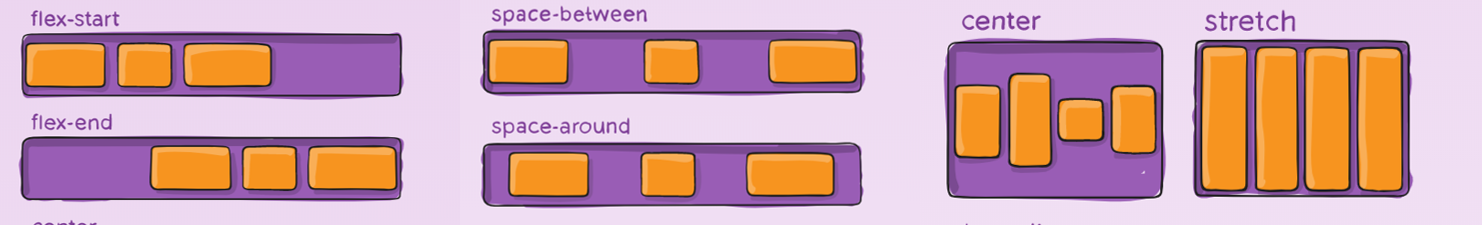
\includegraphics[scale=0.6]{Images/flexbox.png}
    \label{fig:neural_network}
    \caption{Schéma explicatif du fonctionnement des Flexbox sur le site CSS.tricks}
\end{figure}

Le module flexbox nous ainsi permis de disposer nos différents blocs et sections sur notre page, comme nous le souhaitions. \\ Toutefois, lors du premier jet, nous n’avions pas utilisé les balises de structuration introduites par HTML. Nous définissions à chaque fois des classes ou identifiants à nos différents blocs <div>, ce qui alourdissait de manière conséquente notre code HTML ou CSS. \\
L’utilisation, dans un second temps, des balises de structuration HTML,  telles que <header>, <footer>, <nav> ou <section>, délimitant les différentes zones classiques d’une page web, nous a permis de simplifier et structurer le code source et de repérer plus facilement les éventuels erreurs. 


\begin{figure}[H]
    \centering
    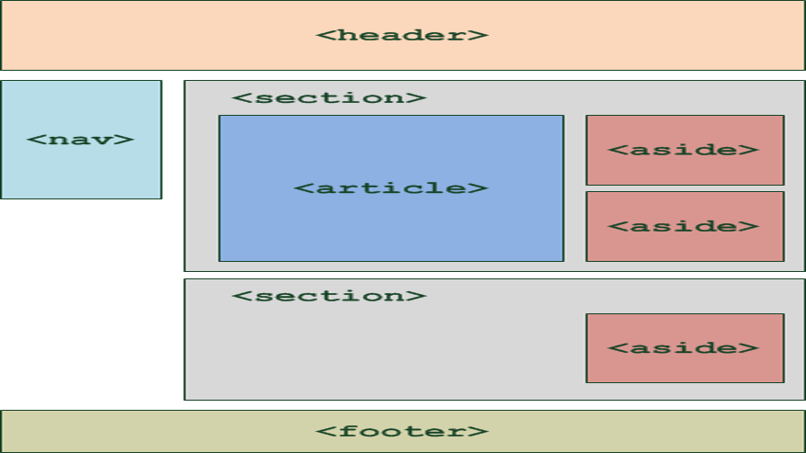
\includegraphics[scale=0.4]{Images/balise.png}
    \label{fig:neural_network}
    \caption{Balises de structuration HTML}
\end{figure}

Ensuite,lors du développement de l'application web, le design et le rendu du site ont été priviligiés, dans un premier temps, devant l'optimalité du code : on se souciait peu des doublons, des redondances et de la longueur du code. Si cela ne posait aucun problème au départ, cela a été conflictuel lors du développement de l'application. Il était alors nécessaire d'effectuer une factorisation du code. \\
La factorisation consiste à trouver les facteurs communs du code pour les regrouper et éviter les répétitions. Cette procédure permet de supprimer les doublons du code CSS et facilite ainsi toute modification du design du siten, en plus de simplifier radicalement le code source. Cette factorisation nous a permis de réduire fortement la longueur du code CSS. 

\medbreak 
Par ailleurs, si ce développement web représente plusieurs avantages, notamment pédagogiques détaillés dans la partie précédente, il possède néanmoins un défaut majeur : il ne possède pas de framework. Des frameworks tels que React Native ou Flutter impose un cadre de travail, une architecture logiciel au développeur et lui fournit diverses bibliothèques. Les requêtes serveur sont alors beaucoup plus simple pour un langage disposant d'un framework. 
Si HTML et CSS sont des langages bien plus universels que Dart ou Swift, ils n'ont pas été pensé pour une éventuelle intégration et les requêtes serveur sont beaucoup plus complexes. Ainsi, une annexe JavaScript a du être rédigée pour relier chacune des requêtes serveur à l'application web.

\medbreak
Enfin, le dernier problème rencontré a été l'homogénéisation du site web. En effet, le développement de l'interface web ayant été effectué par deux personnes différentes, qui étaient tous deux responsables de deux pages différentes, le design des pages n’était pas toujours harmonieux et équilibré. Une mise au point a alors dû être nécessaire pour normaliser l’application web. Cette mise en commun a été rendu possible par l’installation du logiciel GitHub, qui nous a permis de partager le code en temps réel. Les deux frontends ne travaillant pas sur les mêmes pages de l’application, aucun problème de merge conflict a été observé. Nous avons alors pu extraire les meilleurs éléments des deux développement web et nous mettre d'accord sur une charte graphique commune. 
\smallbreak\textit{Rédateur} : Mathieu, \textit{Relecteur} : Nicolas

\subsection{Aperçu du rendu du site et commentaires}

Pour limiter l'accès de l'application aux élèves de l'école et aux membres du personnel, nous avons développé des pages d'authentification. La page login à gauche, permet à un utilisateur possédant déjà un compte sur l'application d'accéder à la page principale. La page register, à droite, permet quant à elle de se créer un compte. Un nouvel utilisateur pourra cliquer sur la flèche en haut à gauche du carré blanc ou sur \textit{sign up} pour accéder à cette page et se créer un compte avec son adresse IMT Atlantique.  Seules les adresses mail avec le suffixe \textit{@imt-atlantique.net} peuvent se créer un compte. 

\begin{figure}[h]
  \begin{subfigure}[b]{0.4\textwidth}
    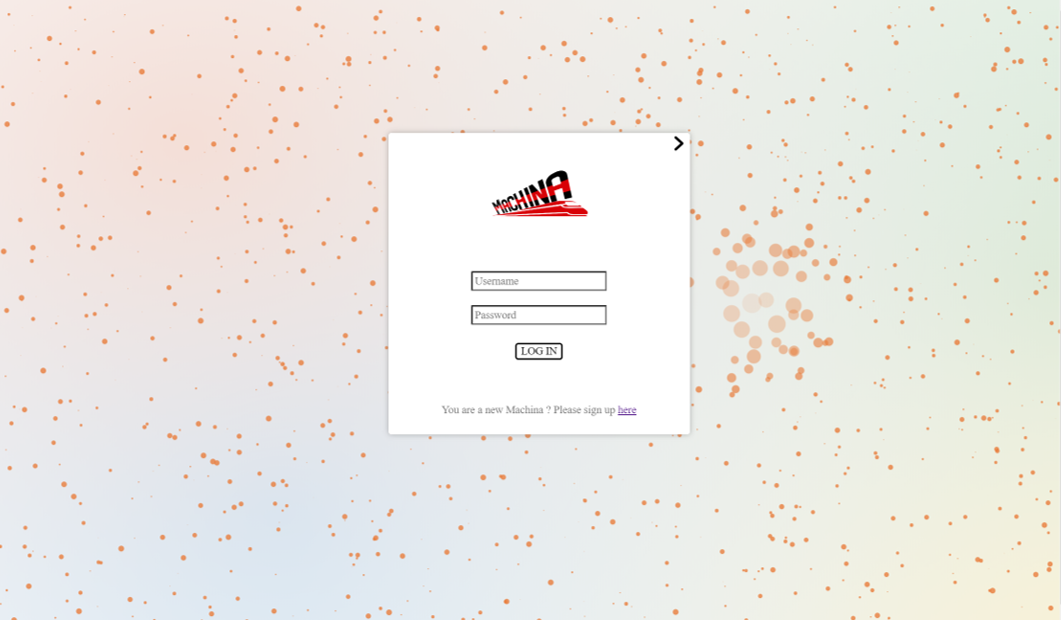
\includegraphics[width=\textwidth]{Images/login.png}
    \caption{Page login}
    \label{fig:f1}
  \end{subfigure}
  \hfill
  \begin{subfigure}[b]{0.4\textwidth}
    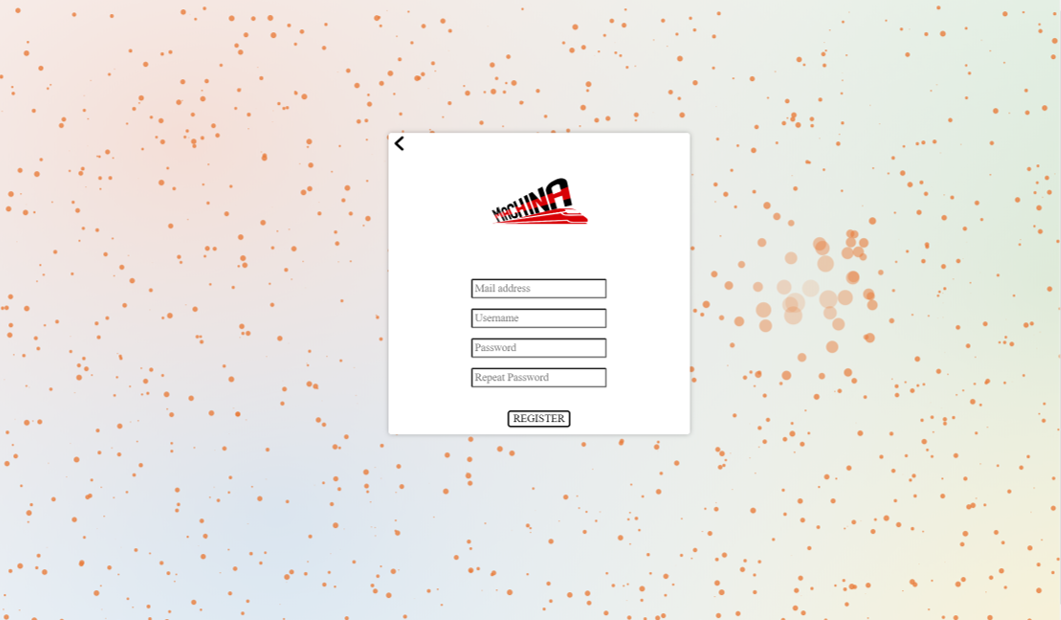
\includegraphics[width=\textwidth]{Images/register.png}
    \caption{Page register}
    \label{fig:f2}
  \end{subfigure}
  \caption{Pages de connection du site}
\end{figure}

La page login permet à l'utilisateur d'accéder ensuite à la page accueil. Cette page (en bas à gauche) est la page principale du site. Elle permet à l'utilisateur de téléverser sur le serveur l'image qu'il souhaite traitée, et la fonction download permet de télécharger sur la machine de l'utilisateur le fichier texte obtenu par l'algorithme de reconnaissance. \\
La partie administrateur, à droite, est une page un peu spécial du site. Il s'agit de la page de gestion du site et seul l'administrateur peut y accéder. Une fois dessus, il peut accéder au statistiques du site et peut contrôler la liste des personnes ayant les accès à l'application. Il peut notamment supprimer une personne présente dans sa base de données pour lui interdire l'accès. 

\begin{figure}[H]
  \begin{subfigure}[b]{0.4\textwidth}
    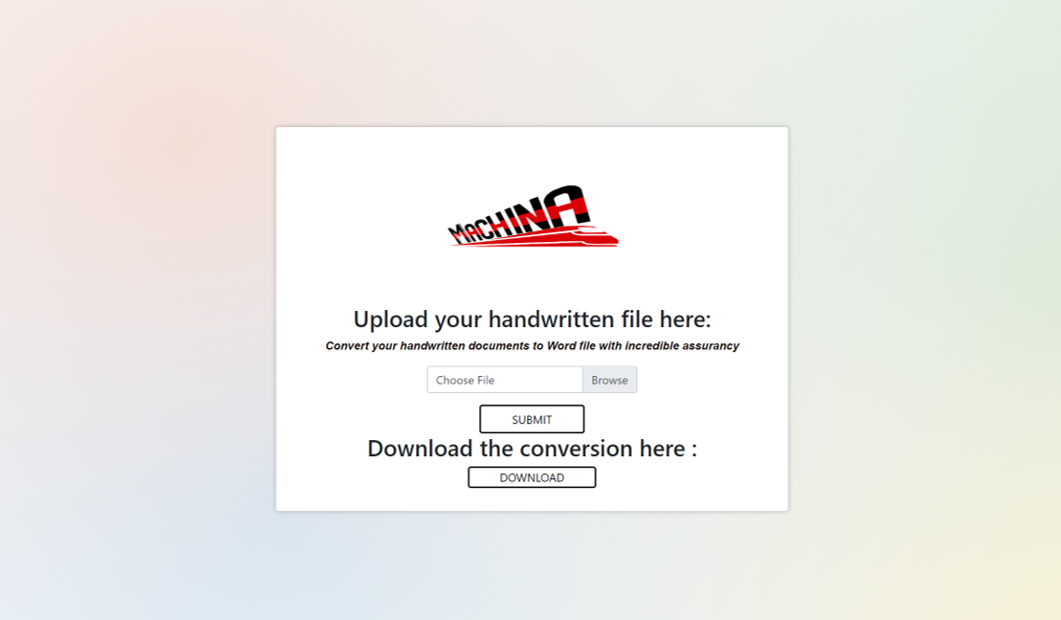
\includegraphics[scale=0.22]{Images/accueil.png}
    \caption{Page accueil}
    \label{fig:f1}
  \end{subfigure}
  \hfill
  \begin{subfigure}[b]{0.4\textwidth}
    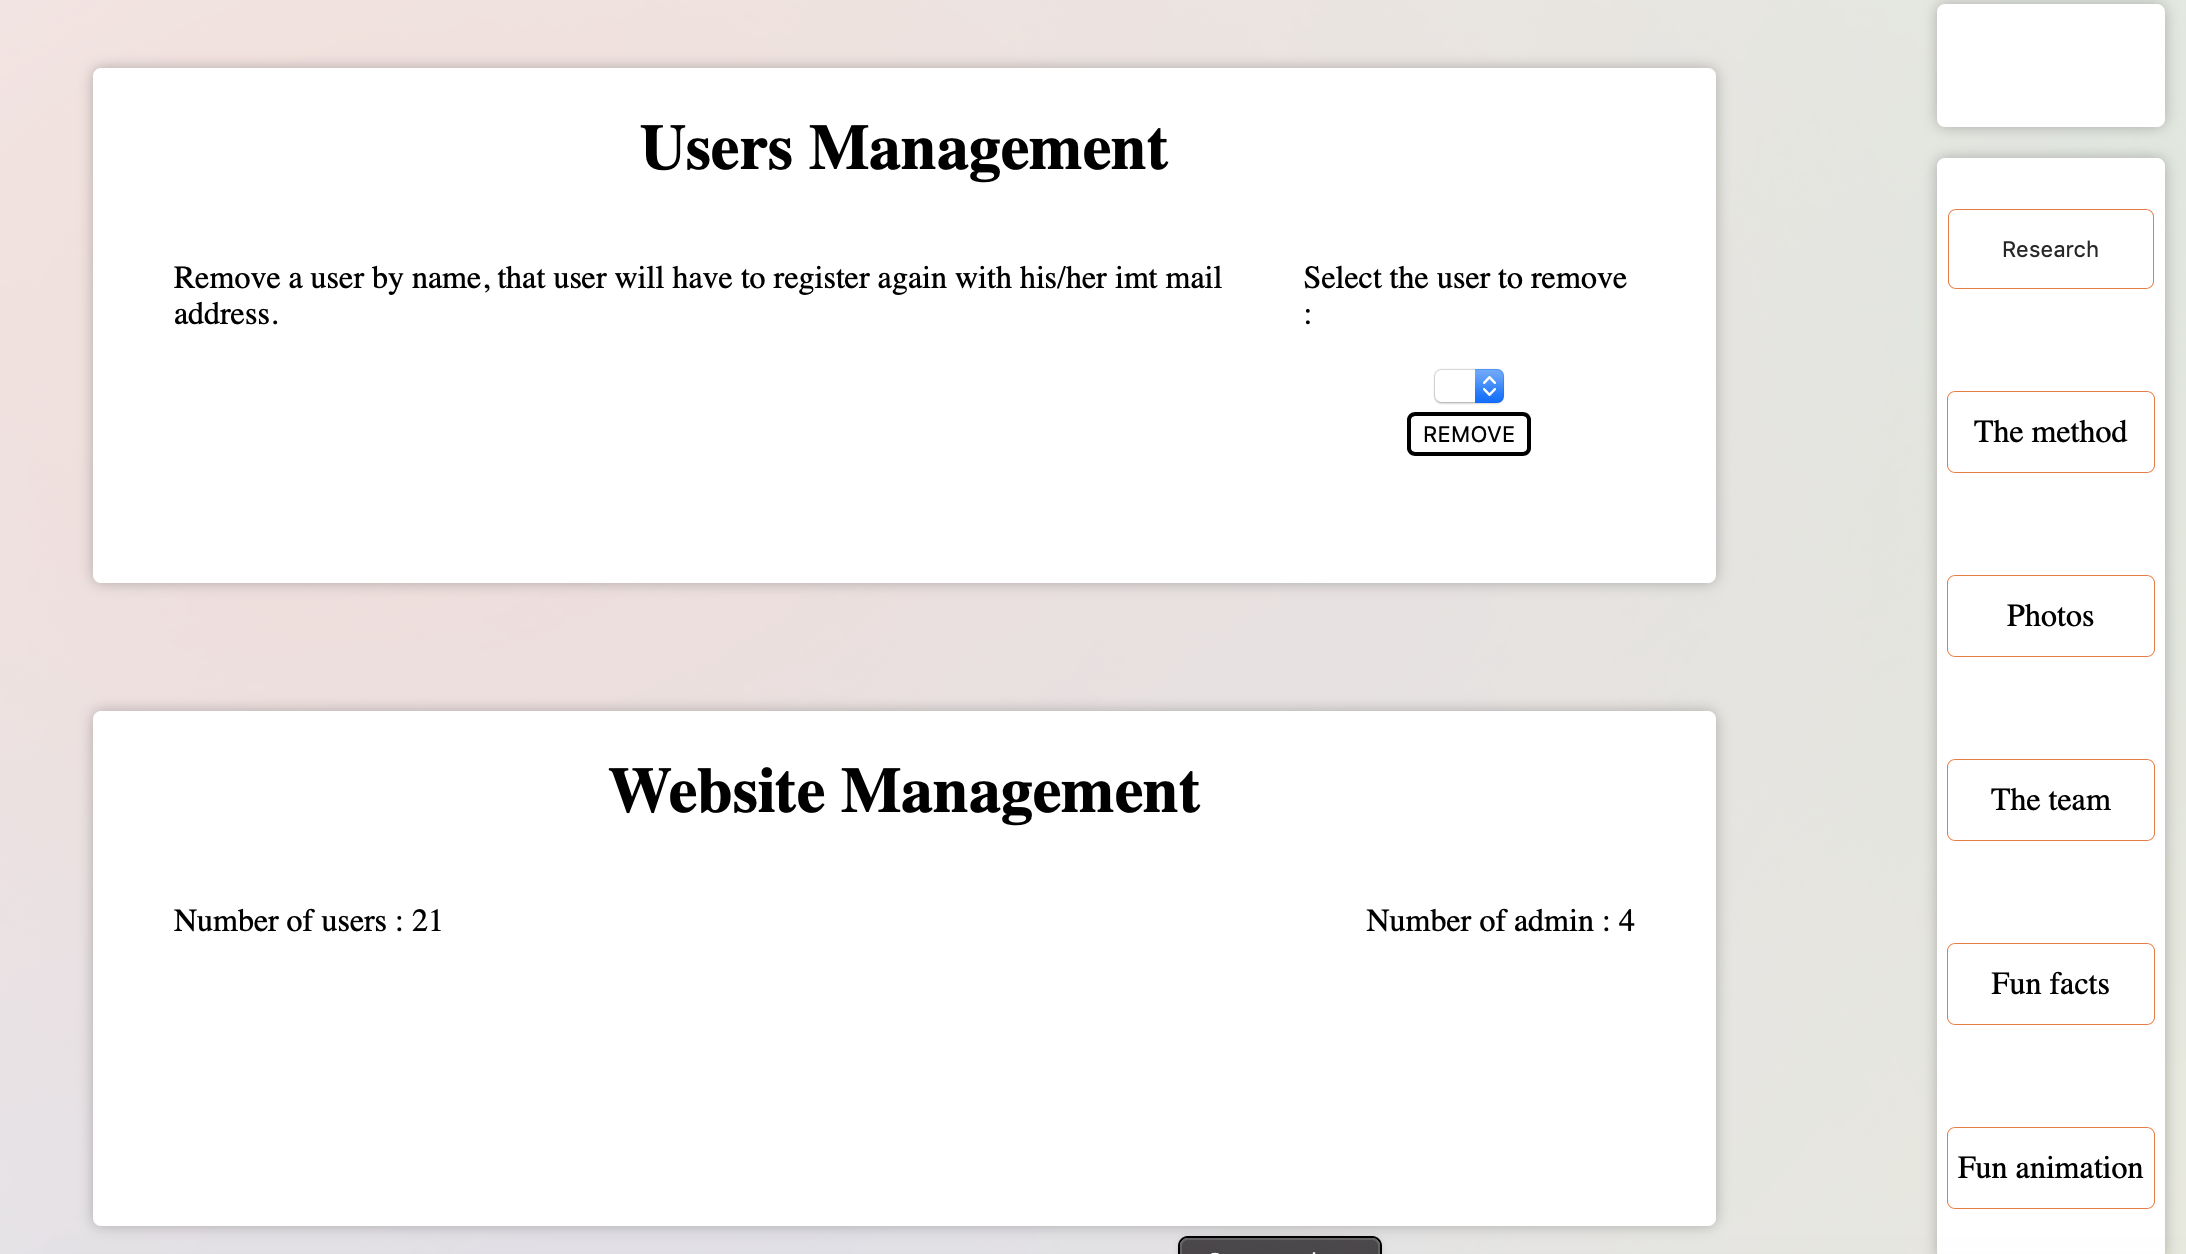
\includegraphics[scale=0.16]{Images/Admin.png}
    \caption{Page administrateur}
    \label{fig:f2}
  \end{subfigure}
  \caption{Pages principales du sites}
\end{figure}

Pour terminer cette partie  Frontend, nous allons décrire plus en détail les fonctions Upload et Download de la page accueil, permettant de faire le lien entre l'utilisateur et le serveur. 
\smallbreak\textit{Rédateur} : Mathieu, \textit{Relecteur} : Nicolas
\subsection{Développement des fonctionnalités Upload et Download}

Une fois que le design et l’architecture de l’application ont été achevés, il fallait relier cette interface web au serveur. En effet, si le frontend améliore l’expérience de l’utilisateur, sans le backend l’application ne serait qu’une coquille vide, un artifice sans utilité. 
\medbreak
Les deux fonctions majeures à développer étaient les fonctions \textit{Upload} et \textit{Download}. 
\\
La fonction \textit{Upload} permet à l’utilisateur d’envoyer une image sous format jpeg ou png au serveur. Une fois déposé sur le serveur, cette image contenant du texte manuscrit pourra être traitée par l’algorithme de reconnaissance et traduite sous format texte. 
A posteriori, le format texte obtenu devra pouvoir être téléchargé par l’utilisateur sur sa console. Une fonction \textit{Download} devra alors être nécessaire. Cette fonction permet cette fois ci d’envoyer le format texte obtenu par l’algorithme de reconnaissance vers la machine de l’utilisateur. 
\smallbreak
Ces deux fonctions sont des requêtes serveur et ne peuvent être réalisées qu’en JavaScript. La fonction permettant de gérer le POST du fichier à uploader doit renvoyer dans le corps de la réponse le fichier texte de la transcription retournée par l'algorithme prévisionnel. Ces deux actions sont asynchrones et doivent être gérée dans une "Promise" qui ne sera terminée que lorsque le réponse sera envoyée au client. Une barre de chargement est affichée pendant toute la durée d'attente entre l'upload et la réception de la réponse. Afin de modifier le corps de la réponse envoyée par le serveur, on ne peut se résoudre à utiliser un simple bloque "form" HTML mais plutôt un script javascript qui est appelé lors de l'envoie du document en cliquant sur le bouton 'Upload'.

\smallbreak\textit{Rédateur} : Nicolas, \textit{Relecteur} : Paul
\section{Backend}

Pour terminer cette partie sur la conception et la réalisation de l'application web, nous allons parler de la partie Backend, partie essentielle, qui donne tout sens au développement Frontend développé précédemment. 
\subsection{Base de donnée}
\subsubsection{MongoDB}

\paragraph{MongoDB en deux mots}
MongoDB est un base de données open-source construite sur une architecture de mise à échelle horizontale. Au lieu de stocker des données dans des tableaux de lignes ou de colonnes comme les bases de données SQL, chaque ligne d'une base de données MongoDB est un document décrit en JSON. \\ 
Pour l'exemple, voici le modele JSON décrivant nos utilisateurs : \\

% \begin{lstlisting}[frame=single]
%   {
%     "_id":"5ea0d40557801a18947562cb",
%     "username":"a",
%     "email":"a@a",
%     "password":"$2a$10$Awv.cB3bQW2cdfZfSCkZ3.
%                 fKi1FAuWjHBehsn9poh0H7HWXZLuqhO",
%     "date": "2020-04-23T07:43:36.791+00:00",
%     "__v": 0
%   }
% \end{lstlisting}

\begin{figure}[H]
    \centering
        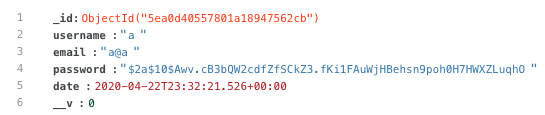
\includegraphics[width=0.8\linewidth]{Backend/Database/User json.png}
        \caption{Modèle d'utilisateur}
        \label{fig:my_label}
\end{figure}

\paragraph{Pourquoi utiliser MongoDB?}
Par construction, ces bases de données de documents sont extrêmement flexibles, permettant des variations dans la structure des documents et permettant le stockage de documents partiellement complets.\\
Comme le montre l'exemple ci-dessus, les champs d'un document jouent le rôle de colonnes dans une base de données SQL et, comme les colonnes, ils peuvent être indexés pour augmenter les performances de recherche.\\
Généralement, MongoDB est utilisé pour intégrer de grandes quantités de données diverses. Dans notre cas, une simple base de donnée mySQL aurait suffit. Cependant, MongoDB étant de plus en plus populaire dans le monde du web developement, notament grace à l'avenement du MEAN stack, nous voulions profiter du projet CODEV pour apprendre cette technologie.

\subsubsection{Atlas et développement collaboratif}

\paragraph{Utilisation en développement}
MongoDB peut être déployé et exécuté sur un ordinateur de bureau, un énorme cluster d'ordinateurs dans un centre de données ou dans un cloud public, soit via MongoDB Atlas, une base de données interactive et collaborative. Cette dernière option nous permet à tous de la consulter et donc de mieux comprendre son fonctionnement. Combiné avec l'outil de développement d'API Postman, ce service permet a chaque membre de l'équipe de tester des requêtes au serveur.

\paragraph{Utilisation en déploiement}
Atlas nous permet de deployer une base de donnée MongoDB sur les clouds d'Amazon (AWS) et de Google (GCP). Disposant de crédits AWS, cette option a été préférée pour le projet. Pour le déploiement, il faudra néanmoins retirer du repository github la clef de connexion privée au compte Atlas.
\smallbreak\textit{Rédateur} : Nicolas, \textit{Relecteur} : Paul
\subsection{Langage et framework}

Depuis son lancement il y a 20 ans, javascript est devenu le langage le plus populaire dans le monde du web developement. C'est un langage qui permet de designer des pages dites dynamiques, dont la construction dépend d'une application serveur, en implémentant des scripts côté client. Dans la pratique, des framework sont utilisés aussi bien au niveau du front-end - Angular, React - que du developpement côté serveur - NodeJS pour javascript, Flask pour python, Cake pour PHP...

\subsubsection{NodeJS}

En un mot, NodeJS utilise des entrées/sorties non bloquante dans l'optique de rester efficace sur des applications en de traitement de donnée en temps réel. Ce framework excelle dans la gestion d'un grand nombre de connexions simultanées, assurant également une certaine flexibilité du réseau. \\
Cependant, NodeJS n'est pas une solution miracle qui domine le monde du web développement. C'est un framework qui répond à des besoins particuliers, il est donc essentiel de bien comprendre son fonctionnement. Comparé aux techniques traditionnelles de serveur web où chaque connexion engendre un nouveau thread, occupant la RAM système et finissant par maximiser la quantité de RAM disponible, Node.js fonctionne sur un seul thread, en utilisant des entrées/sorties non bloquantes, permettant ainsi de supporter des dizaines de millier de connexions simultanées. 

\begin{figure}[H]
    \centering
        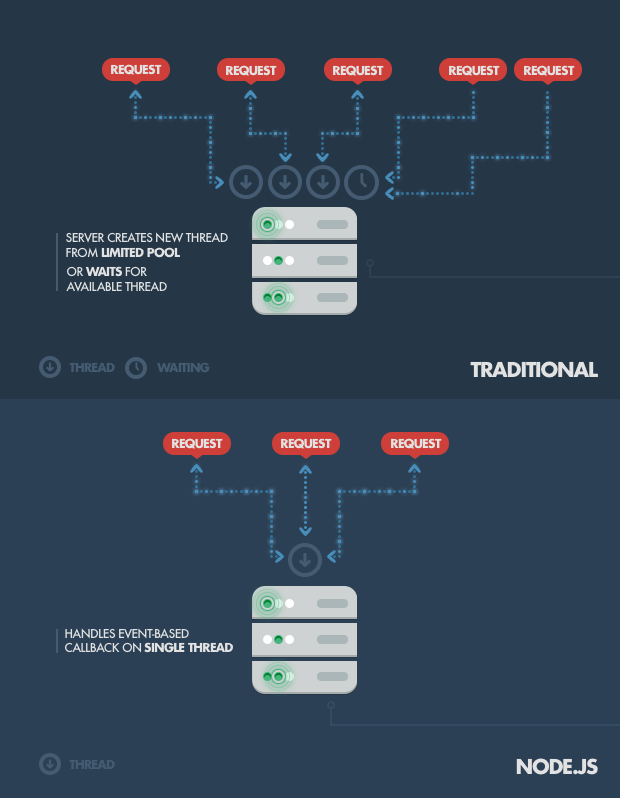
\includegraphics[scale=0.4]{Backend/Lang/NodeJS.png}
        \caption{Principe de NodeJS}
        \label{fig:my_label}
\end{figure}

NodeJS est donc la meilleur option quant au traitement d'un grand débit de donnée. Il serait, par exemple, particulièrement adapté à une application de messagerie en temps réel. \\ \\
Dans le cadre de notre projet, ce framework est utile pour 2 raisons. \\ \\
- Premièrement, il permet d'éviter des conversions multiples de format en utilisation un format uniformisé JSON du client jusqu'à la base de donnée en passant par le serveur. En effet, en utilisant un autre framework, comme Rails, la donnée JSON doit être convertie en modèle binaire après chaque appel du frontend.\\
- Deuxièmement, NodeJS permet la mise en attente des opérations d'écriture et de modification de la base de donnée de manière non-bloquante. Par exemple, dans l'éventualité d'une surcharge d'inscription à un instant t, si les informations des l'utilisateur sont valides - mot de passe de la bonne longueur, email valide, mot de passe validé - il sera immédiatement redirigé vers la page login avant même que ses informations soient enregistrées dans la base de donnée. Cette logique non-bloquante est 
assurée par des "promesses" (promise) et des "fonctions de rappel" (callback). Dans la pratique, cette particularité c'est utile que dans le cas d'une surcharge de donnée à traiter, ce qui ne sera vraisemblablement pas le cas pour notre site. \\ \\

Cependant, l'utilisation de ce framework reste avant tout didactique. Étant de plus en plus populaire, il est important de s'y familiariser le plus tôt possible.

\subsubsection{Node Package Manager}

NodeJS possède un système de management des dépendances : NPM, Node Package Manager. L'idée des modules NPM est assez similaire à celle de Ruby Gems: un ensemble de composants réutilisables et accessibles au public. 

\paragraph{ExpressJS}

Parmis ces packages figure ExpressJS. Express est à NodeJS ce que Boostrap est à HTML/CSS. Afin de comprendre l'utilité de ce package, il est important de comprendre que NodeJS n'est qu'un environnement, un interprète javascript. Il  n'apporte qu'une logique non bloquante et événementielle et ne permet pas, en soit, de configurer un serveur HTTP. \\ \\
C'est la qu'intervient Express, c'est un  module HTTP implémentant des objets usuels comme les cookies ou les sessions. Express introduit également le concept de "routes", associant à un URI un requête. Ainsi, décrire une requête de type POST, GET, DELETE ou PUT depuis un "point d'entrée" peut se résumer à quelques lignes de code. Ce framework simplifie donc grandement la vie du web développeur.  

\paragraph{PassportJS}

Passport est un module d'authentification s'intégrant parfaitement à la logique ExpressJS. Ce package génère automatiquement des objets généralement utiles à l'implémentions d'une phase d'inscription et d'authentification. \\ \\
Pour la partie inscription de cette application web, il a été utilisé pour générer un modèle JSON décrivant chaque utilisateur dans la base de donnée, en automatisant la phase de hashing du mot de passe et l'attribution d'un identifiant unique pour chaque utilisateur. \\
Passport génère également des méthodes et objets utiles à la connexion de l'utilisateur. Par exemple, la persistance de connexion de l'utilisateur est également gérée par ce module, en générant automatiquement un "token" à chaque utilisateur après une connexion. Le token définie une session valide au cours de laquelle l'identification persiste.

\paragraph{MulterJS}

Multer est un des nombreux modules permettant de gérer le téléchargement de document vers le serveur coté client. Basé sur un logique introduite par Busboy, un module NodeJS analysant les données de formulaire HTML entrantes, Multer ajoute automatiquement à la requête envoyée un objet "body" et "file" transmise directement à la base de données. Ce package génère également un modèle JSON des documents importés, pouvant contenir d'autres attributs optionnels comme l'encodage - ici md5.

\smallbreak\textit{Rédateur} : Nicolas, \textit{Relecteur} : Paul
\subsection{Structure}



\subsubsection{Logique MVC}

MVC est un acronyme pour "Model-View-Controller". C'est une norme structurelle divisant le développement en 3 parties distinctes. L'avantage de cette approche est de pouvoir partager les tâches entres développeurs et de maximiser la réutilisabilité du code. Commençons par le premier de ces trois éléments. \\ \\

- \textbf{Modèle} (model): Le modèle représente la structure des données, le format et les contraintes avec lesquelles elles sont stockées. Il maintient les données de l'application. Il s'agit essentiellement de la partie base de données de l'application.\\
Notre base de donnée est constituée de 2 modèles, User, décrivant les utilisateurs enregistrés, et Document, décrivant les documents téléchargés. \\

\begin{figure}[H]
    \centering
        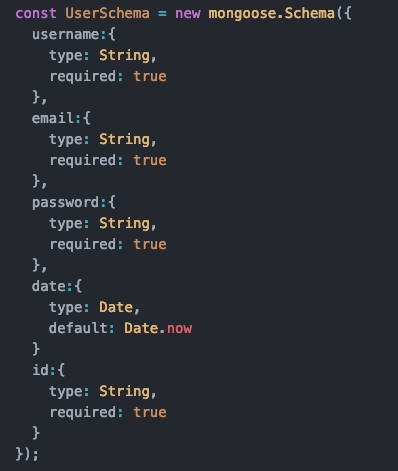
\includegraphics[width=0.3\linewidth]{Backend/Database/user model.png}
        \caption{Modèle d'utilisateur}
        \label{fig:my_label}
\end{figure}

- \textbf{Interface} (view): L'interface est ce qui est présenté à l'utilisateur. Elles utilisent les modèles et présentent les données sous une forme que l'utilisateur souhaite. Cet utilisateur peut également être autorisé à apporter des modifications aux données présentées. Elles se composent de pages statiques et dynamiques qui sont chargées à la demande.\\
Notre site compte 4 interfaces différentes, la page "Login", "Register", "Accueil" et "Admin". \\

- \textbf{Contrôleur} (controller): Le contrôleur contrôle les demandes de l'utilisateur, puis génère une réponse appropriée qui est envoyée au visualiseur. En règle générale, l'utilisateur interagit avec la vue, qui génère à son tour la demande appropriée, cette demande sera traitée par un contrôleur. Le contrôleur affiche l'interface avec les données du modèle comme réponse. \\
Dans la logique NodeJS, les contrôleurs sont les routes. Il y a 5 catégories de routes : login, register, document, admin et accueil. \\

\begin{figure}[H]
    \centering
        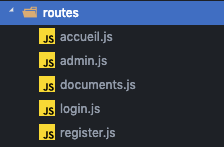
\includegraphics[width=0.3\linewidth]{Backend/Database/routes.png}
        \caption{Organisation des routes (contrôleurs). Chaque fichier contient des gestionnaires d'accès à différents points d'accès.}
        \label{fig:my_label}
\end{figure}

\subsubsection{Architecture}

\begin{figure}[H]
    \centering
        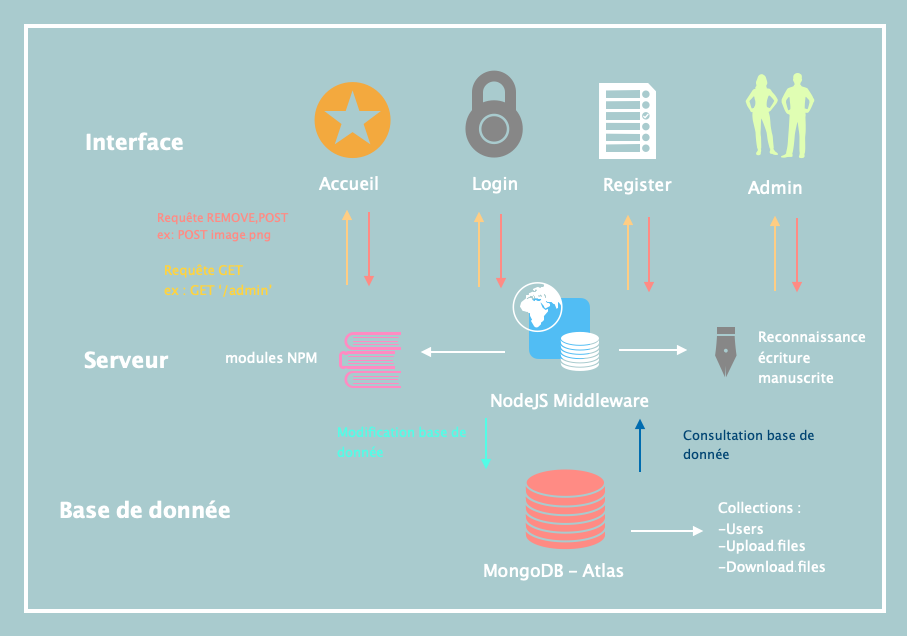
\includegraphics[width=0.8\linewidth]{Backend/Database/Archi.png}
        \caption{Architecture logicielle}
        \label{fig:my_label}
\end{figure}

\smallbreak\textit{Rédateur} : Nicolas, \textit{Relecteur} : Paul
\subsection{Sécurité}

La sécurité est un aspect essentiel du design d'un site web. De l'authentification au stockage des données, des précautions doivent être prises afin d'éviter l'exploitation de vulnérabilités. Sans cela, l'intégrité et la disponibilité des données et du site ne sont pas assurées. \\
Dans cette partie, les mesures prises seront détaillées au niveau de la communication client-serveur, du stockage des données et de la navigabilité du site. Par soucis d'honnêteté, les failles de sécurité persistantes seront également présentées.

\subsubsection{Stockage des données}

\paragraph{Utilisateur}

Chaque utilisateur est enregistrée dans la base de donnée MongoDB dans la collection "users". Les données d'identification, identifiant et mot de passe, sont confidentielles et doivent donc être protégées. \\
La règle d'or pour assurer leurs protections est de ne rien stocker en clair dans la base de donnée. Il faut donc encrypter la donnée avant de l'enregister. Les fonctions de hashage permettent l'encryption unilatérale de la donnée puisque leurs réciproques est indéterminable (ou presque). \\ \\
Lors de l'inscription d'un nouvel utilisateur, le mot de passe est hashé par une fonction basée sur l'algorithme de cryptographie SHA-1. Le mot de passe en clair n'est donc pas renseigné sur le base de donnée, l'identification se fait donc en comparant le hash du mot de passe enregistré et celui obtenu lors de chaque tentative d'identification de l'utilisateur. En pratique, l'encryption est effectuée à partir des méthodes randomBytes() et compare() des objets "crypto" du module passeport.\\ \\
Ne pas hasher le mot de passe des utilisateur rend le site vulnérable aux injections SQL si la base de donnée est écrite en SQL, et plus généralement aux attaques d'ingénierie sociales résultant à l'accès de la base de donnée par l'attaquant. \\ \\
Néanmoins, l'encryption des données reste partielle. En effet, seul le mot de passe l'est, il faudrait faire de même pour l'identifiant et l'adresse email. De plus, l'algorithme de hashage SHA-1 reste vulnérable puisqu'une brèche de sécurité nommée SHAterred a été exhibé en 2017 par Google et par le CWI (Centrum Wiskunde and Informatica). Un risque bien plus préoccupant reste la vulnérabilité du site aux attaques par dictionnaire puisqu'il n'y a aucune limite de tentative de connexion par IP. 

\paragraph{Documents}

Chaque document téléchargé sur le serveur est également encrypté par la fonction de hash md5. Cette fonction est certes moins robuste que SHA-1 mais la donnée est considérée comme moins sensible. Leur est également associé un identifiant unique afin d'éviter des doublons dans la base de donnée. \\ \\
Un attaquant pourrait potentiellement exploiter une référence directe de chaque document dans l'url. En effet, dans les premières version du site, l'utilisateur était redirigé vers un url contenant l'identifiant unique de son document. Connaissant cet identifiant, l'accès au document n'est potentiellement plus protégée. Cette faille à néanmoins  été corrigée, il n'y a plus de redirection mais plutôt un téléchargement in-situ de la transcription à partir d'un bouton "Download" situé sur la page principale.

\begin{figure}[H]
    \centering
        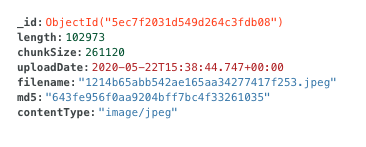
\includegraphics[width=0.5\linewidth]{Backend/Database/documents schema.png}
        \caption{Modèle des documents téléchargés à partir du client sur le serveur}
        \label{fig:my_label}
\end{figure}


\subsubsection{Navigation et communication}

\paragraph{Navigabilité et restriction}

L'accès à différents URL et fonctionnalité dépend de l'état de l'utilisateur : visiteur, authentifié, admin. Il est donc important d'effectuer des tests d'accessibilité du contenue tout au long de la navigation. \\ \\
Dans la pratique, une fonction de vérification de statut est appelé à chaque requête vers du contenu protégé. Cette fonction renvoie le statut de l'utilisateur à chaque appel. Le statut visiteur donne accès aux routes "/login"et "/register", le statut authentifié donne accès à la route '/' - page d'accueil - et à toutes ses fonctionnalités - "Upload" et "Download" des documents, enfin le statut admin donne accès aux routes '/' et '/admin' et à toutes leurs fonctionnalitées. Ainsi les membres authentifiés ne peuvent plus accéder a la page d'authentification, et les visiteurs ne peuvent pas accéder à la page d'accueil. \\ \\
Sans cette phase de vérification, un utilisateur non autorisé, non étudiant à l'IMT Atlantique par exemple,  pourrait accéder à des fonctionnalités protégées.

\paragraph{Protocole HTTPS}

Le protocole de communication HTTPS repose sur un certificat d'authentification du visiteur d'un site site certifié par certificat SSL délivré par la une autorité tiers comme IdenTrust ou DigiCert. Il permet d'assurer la légitimité de la communication instanciée par le visiteur, en empêchant une attaque dite de l'homme du milieu. \\ \\
Dans la pratique, instaurer ce protocole de communication n'est utile qu'au déploiement du site. En phase de développement, HTTP est le protocole que nous avons utilisé. Obtenir un certificat SSL n'est possible qu'après avoir réservé un nom de domaine, ce qui n'est pas notre cas. Cependant, acquérir ce certificat est une priorité quant à la sécurité des échanges client-serveur, le déploiement ne se fera donc qu'avec un certificat SSL.

\smallbreak\textit{Rédateur} : Nicolas, \textit{Relecteur} : Paul
\section{Validation}

Pour terminer ce rapport, nous allons essayer de prendre un peu de recul sur les résultats obtenus et les choix faits durant ce projet. 
\subsection{Retour sur les choix effectués}
Dans cette partie nous allons développer les choix qui ont été effectués notamment pour la réalisation du modèle d'apprentissage profond, des bases de données utilisée, des réseaux de neurones implémentés, des fonctions de normalisation et d'activation utilisées, etc... .\\
\medbreak
\textbf{Choix de la base de donnée} : Nous nous sommes tout d'abord penché sur la base de données \textbf{Chars74k} qui est une base de données de lettres photographiées sur google street. Le choix de cette base de données fut une erreur car après plusieurs tentatives, l'algorithme était dans l'incapacité de prédire des mots entiers, ce fût donc notre premier échec et nous en développerons les raisons plus précisément dans la section \textit{écueil à éviter}. Cette erreur nous a conduit à nous intéresser aux base de données répertoriant des mots. Deux bases de données ressortaient régulièrement dans les articles traitant de reconnaissance manuscrite : la base de données française \textbf{RIMES} et la base de données anglaise \textbf{IAM}. Notre choix à porté sur la base de données anglaise car nous ne trouvions pas de décodeur pertinent en français ce qui réduit dramatiquement les performances.
\medbreak
\textbf{Choix de la structure du réseau de neurones}
La structure de la base de données est entièrement inspirée d'un projet déjà existant, le fait de reprendre une architecture abouti permettait de se concentrer sur les aspect techniques et le fonctionnement des différents types de réseaux neuronal plutôt que de se pencher sur des problèmes purement informatique. Nous avons donc utilisé l'architecture suivante [5] :
\begin{figure}[H]
    \centering
        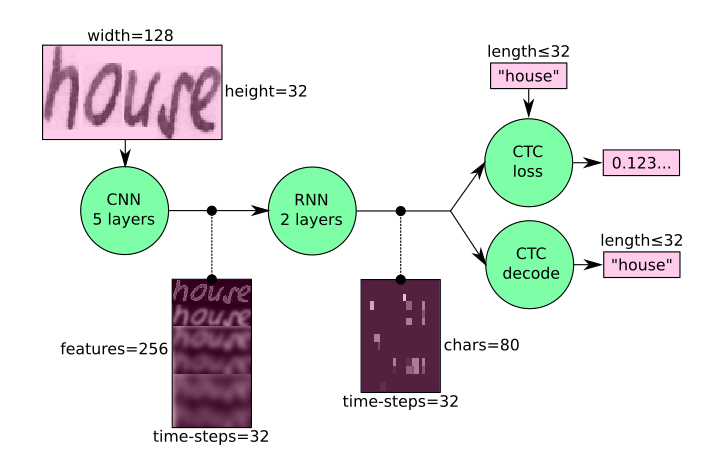
\includegraphics[width=0.8\linewidth]{Images/architecture.PNG}
        \caption{Architecture du réseau de neurone}
        \label{fig:my_label}
\end{figure}
Ainsi le réseau est composé de 5 réseaux à convolutions de 2 réseaux de neurones récurrents. Le fonctionnement de ces types de structure est développé en annexe.
\medbreak
\subsection{Conseil d'optimisation}
\textbf{Conseil pour les améliorations à apporter sur le modèle d'apprentissage profond} : \\
Le modèle utilisé est loin d'être parfait et mériterait qu'on l'améliore. Tout d'abord, l'augmentation de la définition (et donc de la taille) des images permet le nombre de pixel et donc la précision de l'algorithme. Un deuxième conseil pour améliorer les performances pourrait être de supprimer le style d'écriture des textes présent sur les images. Enfin, augmenter le nombre de réseaux à convolution où utiliser des réseaux de neurones récurrents bidirectionnel pourrait également permettre de faire de meilleurs prédictions.

\subsection{Les écueils à éviter}
Notre première erreur et celle qui nous a coûté sûrement le plus de temps a été de réserver certaines tache à des membres. En effet nous pensions gagner du temps en allouant le travail de backend à un membre et le travail de machine learning à un autre pensant que leurs compétences dans ces domaines les feraient progresser plus rapidement que d'autres. Mais sur un projet,il est difficile de se remettre en question seul. La crise sanitaire n'a pas arranger les choses et la mise en commun et le travail en groupe furent très compliqués à mettre en oeuvre. Le conseil que nous pourrions donner serait de travailler sous-groupe au sein du même groupe sur des taches identiques même si la différence de niveau ou de compétence peut paraître handicapante à première vue.\\
La seconde erreur a été une relecture de notre code et des tests d'intégration trop peu réguliers. En effet le debogage d'un code de plusieurs centaines de lignes peut s'avérer très fastidieux et représenter une perte de temps considérable. Il ne faut pas hésiter à tester son code après l'ajout de quelques lignes même si celle-ci ne paraissent poser aucun problème.
\smallbreak\textit{Rédateur} : Nicolas, \textit{Relecteur} : Hugo


\section{Conclusion}
Dans le cadre de notre projet Codev, nous devions développer une application permettant aux élèves de IMT Atlantique de convertir une photo contenant du texte manuscrit sous format numérique. Si aujourd'hui l'application n'est pas prête au déploiement, le développement web est presque terminé. \\
L'utilisateur peut dès à présent téléverser une image sur le site, télécharger sur son ordinateur le fichier texte obtenu par l'algorithme de reconnaissance manuscrite et se connecter sur l'application via son adresse mail. La page de connection n'est pour le moment pas reliée à une base de données des élèves et membres du personnel de IMT Atlantique mais tout élève ne possédant pas le suffixe \textit{@imt-atlantique.net} dans son adresse mail ne pourra se connecter. La page pourrait éventuellement être reliée ultérieurement à une base de donnée IMT Atlantique pour réserver son accès exclusivement aux membres de l'école et respecter le protocole de sécurité imposé dans les contraintes. \\
De plus, nous avons réussi à mettre au point un algorithme de reconnaissante manuscrite mais sa précision ne respecte pas les conditions de validation du cahier des charges. Pour l'intégration, nous avons alors utilisé une API Google, pour résoudre notamment les problèmes de compatibilité avec MAC. 

\medbreak
Si ce projet n'est pas totalement achevé, nous avons conçu l'application de manière à ce qu'elle soit maintenable au possible et que le projet puisse être repris et terminé. Il faudrait notamment essayer de d'améliorer l'algorithme de reconnaissance pour l'intégrer à l'application. Pour améliorer l'expérience de l'utilisateur, il serait également utile de renvoyer un fichier Word modifiable à la place d'un fichier texte et stocker les différents documents traduits par l'application sur le compte de l'utilisateur.  

\medbreak
Enfin, nous voulions juste préciser que ce projet de reconnaissance manuscrite n'était pas le projet initial. Nous souhaitions au départ utiliser des outils de Machine Learning pour prédire le prix des billets de train. En raison de l'épidémie du Covid19, nous n'avions pas réussi à obtenir une base de données assez importante par webscrapping pour effectuer un quelconque modèle de prédiction. Néanmoins, tout a été pensé pour une potentielle reprise du projet : l'application est sécurisée pour éviter son blocage par la SCNF, le code de webscrapping pour extraire les prix quotidiens des trains Paris/Brest et Paris/Nantes est fonctionnel , et la page web a un design similaire au projet initialement prévu.  

\medbreak
Pour conclure, malgré les nombreux rebondissements, ce projet ambitieux nous a permis d'acquérir de nombreuses connaissances techniques, notamment en Machine Learning et en développement web, et des connaissances humaines avec le travail en groupe. Ce projet nous a ainsi été très enrichissant et nous a permis de remplir de multiple objectifs. 

\smallbreak\textit{Rédateur} : Mathieu, \textit{Relecteur} : Nicolas


\section{Annexes}
\subsection*{Réseaux de neurones à convolution}
Les réseaux de neurones à convolution (CNN) désignent une sous-catégorie de réseaux de neurones spécialisé dans la reconnaissance d'image. Sa particularité est sa capacité à reconnaître des motifs dans une donnée ce qui est très pratique dans le cas de la reconnaissance de patternes dans une image.\\ \\
La structure d'un CNN est spécifique à son fonctionnement, elle est composée principalement de deux blocs :
La fonction du premier bloc est l'extraction d'objet appelée \emph{Features maps} par des opérations de filtrage (opération de convolution). La convolution est une opération mathématique qui consiste à assembler deux sets d'information. Dans le cas des réseaux de neurones à convolution, nous appliquons un filtre de convolution pour produire une feature map. Le principe est de faire "glisser" le filtre de convolution aussi appelé couramment \emph{Kernel}, sur l'image d'entrée. Pour chaque position, l'opération AND est réalisé entre le filtre et l'image et le résultat renvoyé est le nombre de bit égal à 1. La feature map est constituée après que le filtre soit passé par toutes les positions.
\begin{figure}[H]
    \centering
        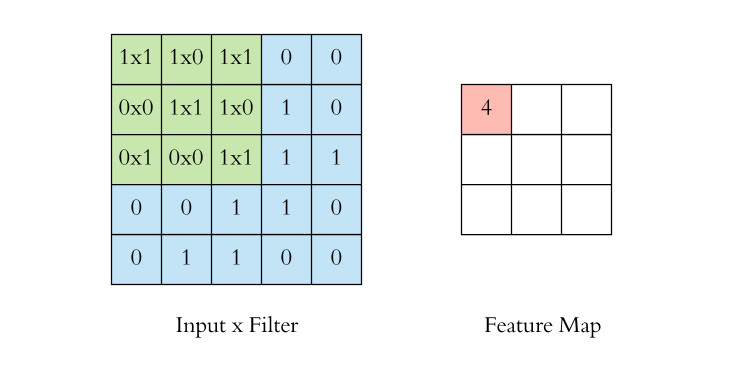
\includegraphics[width=0.7\linewidth]{Images/Convolution.PNG}
        \caption{Opération de convolution entre une image et un filtre}
        \label{fig:my_label}
\end{figure}
Sur la figure 10, on voit donc qu'on applique un filtre 3x3 sur l'image d'entrée et que uniquement 4 de cette image correspondent aux critères du filtre. L'exemple fourni est donc une illustration d'un réseau de neurones à convolution en 2D, mais il existe des réseaux convolutifs qui prennent en entrée des données en 3D.\\
Enfin, dans l'extrême majorité des cas, le réseaux est implémenté pour extraire plusieurs features map d'une seul image à partir de plusieurs filtres. Après avoir extrait ces features map, le CNN se charge de les concaténer et les transformer en input pour une prochaine couche de neurones.\\ \\
La seconde opération est appelée \emph{Pooling}, elle consiste principalement à réduire les dimensions d'une input (en général issue de la concaténation des feature maps) dans le but de réduire la durée d'entraînement et de prévenir les phénomènes d'overfitting. Pour une opération de pooling, on définit d'abord une fenêtre de pooling (hauteur, largeur) ainsi qu'un pas, qui indique comment se déplace la fenêtre sur l'image. L'opération la plus commune est le \emph{Max-pooling} qui consiste à extraire la plus grande valeur de la fenêtre de pooling.
\begin{figure}[H]
    \centering
        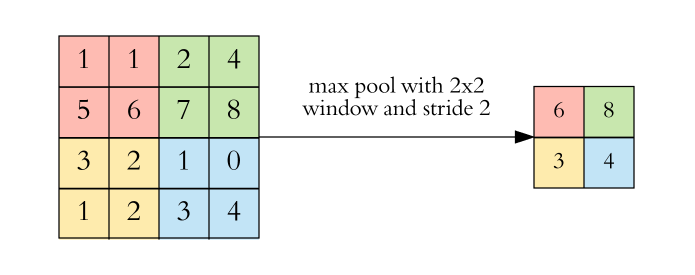
\includegraphics[width=0.8\linewidth]{Images/pooling.PNG}
        \caption{Opération de pooling sur une donnée}
        \label{fig:my_label}
\end{figure}
Sur la figure ci-dessus, on réalise une opération de max-pooling avec une fenêtre de 2x2 et un pas de 2.
Dans un réseau de neurone profond il est très commode de faire suivre à un réseau de neurones convolutif des couches de neurones standards présentées précédemment. En effet un CNN ne suffit pas pour traiter des données efficacement, la forme du résultat en sortie de pooling n'étant pas en général celle attendue.\\ \\
Enfin, un algorithme de convolution est appliqué pour reconnaître des motifs propre à chaque lettres de l'alphabet grec.[6]
\smallbreak\textit{Rédateur} : Hugo, \textit{Relecteur} : Mathieu
\subsection*{Réseaux de neurones récurrents}
Les réseaux de neurones récurrents (RNN) sont intéressant comparés aux réseaux de neurones standards dans le sens où ils permettent de traiter les données en "séries". Un réseau de neurones classiques prend en entrée une donnée de taille fixe, une image de taille (x,y) par exemple, mais comment traiter le cas de phrase, quelle serait le cas d'un algorithme d'apprentissage profond qui ne serait capable de traduire uniquement des phrases de taille fixe d'un langue à une autre. Ainsi un réseau de neurones récurrents prend en paramètres des entrées sans taille prédéterminée.\\
Un RNN est donc idéal pour le traitement de données entrantes sous formes de séries comme par exemple une suite de lettres dans notre exemple. En effet la particularité du RNN est de se souvenir du passé au sein d'une même couche de neurones :
\begin{figure}[H]

\begin{subfigure}{0.5\textwidth}
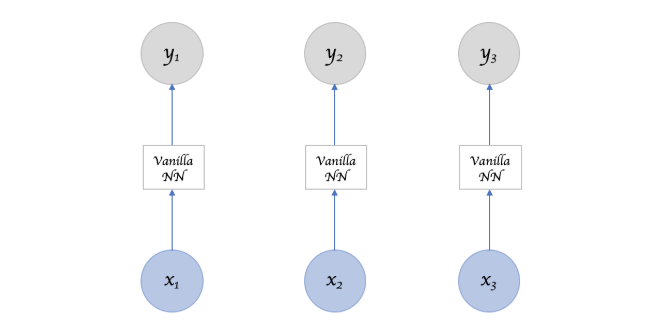
\includegraphics[scale=0.4]{Images/vanilla.PNG} 
\caption{couche de neurones standard}
\label{fig:subim1}
\end{subfigure}
\begin{subfigure}{0.5\textwidth}
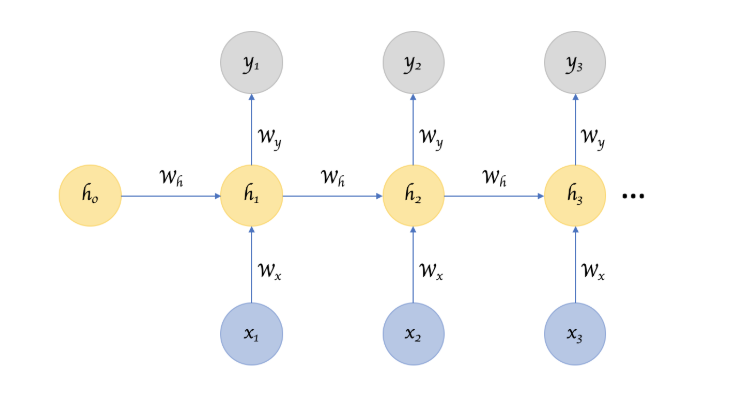
\includegraphics[scale=0.4]{Images/RNN.PNG}
\caption{couche de neurones récurrent}
\label{fig:subim2}
\end{subfigure}

\caption{Différence structurel entre un réseau de neurone standard et un réseau de neurone récurrent}
\label{fig:image1}
\end{figure}
Ainsi, une même entrée peut produire différentes sorties selon les entrées précédentes dans la série. Dans un réseau de neurones standard, un vecteur de taille fixe est transformé en second vecteur de taille fixe contrairement à un réseau de neurones récurrents, où une série d'entrée est transformée en une seconde série de taille quelconque.\\ \\
Durant la phase d'entraînement, de la même façon que pour un réseau de neurones classique, l'objectif est de diminuer la valeur d'une certaine fonction coût et de modifier les paramètres Wh, Wx, Wy... comme indiquée sur la figure 12 (b).\\ \\
Enfin, dans le domaine de la reconnaissance manuscrite, les réseaux de neurones récurrents sont très commode pour mémoriser les fréquences d'apparition de certaines suites de caractères, comme par exemple "ette" en français ou "ye" en anglais. et ainsi d'éviter l'écueil qui consisterait à prédire chaque lettre une à une.[7]
\smallbreak\textit{Rédateur} : Hugo, \textit{Relecteur} : Mathieu
\subsection*{Fonction de normalisation}
Le but de cette partie est d'apporter quelques renseignements supplémentaires sur les fonctions de normalisation et de standardisation les plus usuelles :
\paragraph{Z Normalisation - Standardisation}
\smallbreak
Une normalisation est une transformation linéaire qui transforme des données pour obtenir une moyenne de 0 et un écart-type de 1.
\begin{equation}
z_{i} = \frac{x_{i}-\bar{x}}{s}
\end{equation}
Avec $x_{i}$ les entrées, $\bar{x}$ la moyenne et s l'écart-type.
\paragraph{Min-Max Normalisation}

Une normalisation vise à dimensionner les données entre 0 et 1 sans menacer leur intégrité.
\begin{equation}
\hat{x_{i}} = \frac{x_{i}-x_{min}}{x_{max}-x_{min}}
\end{equation}
Avec $x_{i}$ les entrées, $x_{min}$ et $x_{max}$ respectivement les valeurs minimal et maximal du vecteur $x_{i}$.\\ \\
\smallbreak\textit{Rédateur} : Hugo, \textit{Relecteur} : Mathieu
\subsection*{Fonction d'activation}
\paragraph{Sigmoïde}
Le but de la fonction sigmoïde est de réduire la valeur d'entrée entre 0 et 1, ce qui peut être commode pour exprimer une valeur sous forme de probabilité. L'avantage de cette fonction est que seul les valeurs centrées proche de 0 influent fortement sur la valeur de sortie, ce qui permet d'exclure automatiquement les extremas.

\begin{equation}
    \sigma(x) = \frac{1}{1 + \exp{(-x)}}
\end{equation}
\begin{figure}[H]
    \centering
        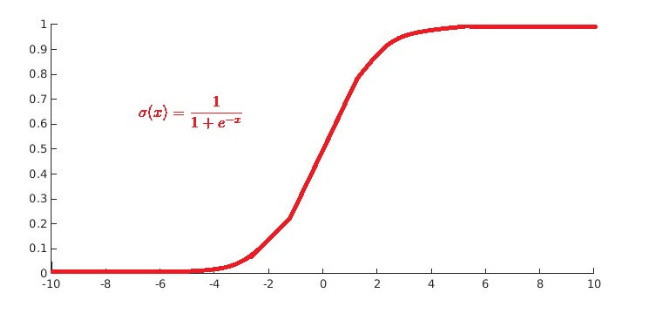
\includegraphics[width=0.8\linewidth]{Images/sigmoide.PNG}
        \caption{Fonction Sigmoïde}
        \label{fig:my_label}
\end{figure}
Les principaux défauts de la fonction sigmoïde sont qu'elle n'est pas centrée en zéro et qu'elle est très coûteuse en calcul.\\ \\
\paragraph{Tangente hyperbolique}
La fonction tangente hyperbolique appelée tanh est semblable à la fonction sigmoïde à l'exception qu'elle renvoie un résultat compris entre -1 et 1. Cependant elle est préférée à la fonction sigmoïde car elle est centrée en zéro [8].
\begin{equation}
    tanh(x) = \frac{\exp{x} - \exp{-x}}{\exp{x} + \exp{-x}}
\end{equation}
\begin{figure}[H]
    \centering
        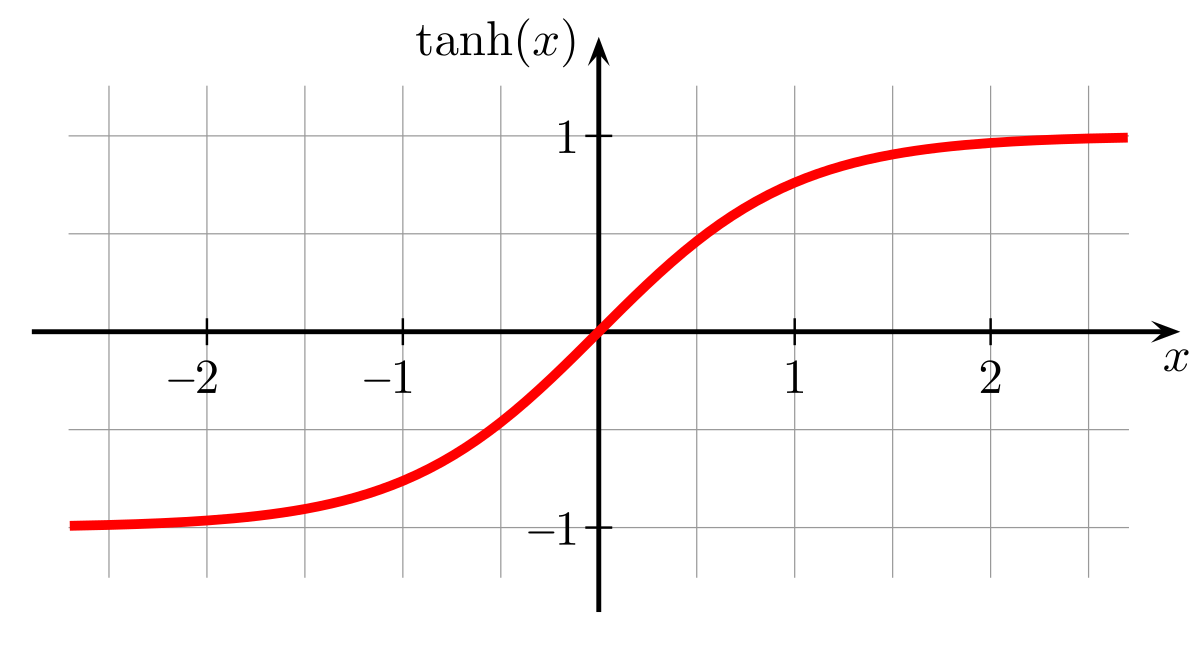
\includegraphics[width=0.8\linewidth]{Images/tanh.png}
        \caption{Fonction tangente hyperbolique}
        \label{fig:my_label}
\end{figure}
\smallbreak\textit{Rédateur} : Hugo, \textit{Relecteur} : Mathieu
\subsection*{Liste des dépendances NodeJS}

acorn: 7.1.1, 
    bcrypt: 4.0.1, 
    bcryptjs: 2.4.3, 
    bull: 3.13.0, 
    bull-board: 0.7.0, 
    child_process: 1.0.2, 
    clean-css: 4.2.3, 
    connect-mongo: 3.2.0, 
    constantinople: 4.0.1, 
    cors: 2.8.5, 
    crypto: 1.0.1, 
    express: 4.17.1, 
    express-flash: 0.0.2, 
    express-flash-messages: 0.1.1, 
    express-session: 1.17.1, 
    gridfs-stream: 1.1.1, 
    html: 1.0.0, 
    log4js: 6.2.0, 
    method-override: 3.0.0, 
    mongoose: 5.9.9, 
    morgan: 1.10.0, 
    multer: 1.4.2, 
    multer-gridfs-storage: 4.0.3, 
    npm: 6.14.4, 
    passport: 0.4.1, 
    passport-local: 1.0.0, 
    rotating-file-stream: 2.0.2, 
    secret: 1.0.2, 
    session: 0.1.0

\section{Glossaire}
\textbf{Apprentissage profond} : Le deep learning ou apprentissage profond est un type d'intelligence artificielle dérivé du machine learning (apprentissage automatique) où la machine est capable d'apprendre par elle-même, contrairement à la programmation où elle se contente d'exécuter à la lettre des règles prédéterminées.
\medbreak
\textbf{Backend} : Le Back-End correspond à la partie immergée de l'iceberg. Elle est invisible pour les visiteurs mais représente une grande partie du développement d'un projet web. Sans elle, le site web reste une coquille vide. Elle est composée d'un serveur, d'une application et de bases de données. 
\medbreak
\textbf{Bounfing Boxes} : Les "bounding boxes" sont des boîtes englobantes imaginaire permettant de définir les contours d'un objet.
\medbreak

\medbreak
\textbf{Cake} : CakePHP est un framework web libre écrit en PHP distribué sous licence MIT. Il suit le motif de conception Modèle-Vue-Contrôleur et imite le fonctionnement de Ruby sur Rails.

\medbreak
\textbf{Callback} : Une fonction callback est une fonction passée à une autre fonction en tant qu'argument, qui est ensuite invoquée à l'intérieur de la fonction externe pour terminer une sorte de routine ou d'action.

\textbf{Code source} : code écrit dans un langage de programmation et qui peut être converti pour constituer un programme exécutable.

\medbreak
\textbf{Charge CPU} : Le niveau de la charge CPU indique l'intensité avec laquelle le processeur traite les programmes et les processus en cours d'exécution.

\textbf{CWI} : Le Centrum voor Wiskunde en Informatica (CWI) (néerlandais pour « Centre pour les mathématiques et l'informatique ») est un centre de recherche national en mathématiques et informatique à Amsterdam, aux Pays-Bas.

\medbreak
\textbf{Descente de gradient} : L'algorithme du gradient désigne un algorithme d'optimisation différentiable. Il est par conséquent destiné à minimiser une fonction réelle différentiable définie sur un espace euclidien.
\medbreak

\medbreak
\textbf{Flask} : Flask est un framework open-source de développement web en Python. Son but principal est d'être léger, afin de garder la souplesse de la programmation Python, associé à un système de templates.

\textbf{Framework} : Un framework est, comme son nom l’indique en anglais, un “cadre de travail“. L’objectif d’un framework est généralement de simplifier le travail des développeurs informatiques (les codeurs si vous préférez), en leur offrant une architecture “prête à l’emploi” et qui leur permette de ne pas repartir de zéro à chaque nouveau projet.
\medbreak
\textbf{Fonction d'activation} : Dans le domaine des réseaux de neurones artificiels, la fonction d'activation est une fonction mathématique appliquée à un signal en sortie d'un neurone artificiel.
\medbreak
\textbf{Frontend} : La partie Frontend correspond aux éléments du site que l'on voit à l'écran et avec lesquels on peut interagir. 

\medbreak
\textbf{Hybride} : Une application hybride est une application utilisant le navigateur web intégré du support (Smartphone ou tablette) et les technologies Web (HTML, CSS et Javascript) pour fonctionner sur différents OS (iOS, Android, Windows Phone, etc.).

\medbreak
\textbf{HTTPS} : L'HyperText Transfer Protocol Secure (HTTPS, littéralement « protocole de transfert hypertextuel sécurisé ») est la combinaison du HTTP avec une couche de chiffrement comme SSL ou TLS.

\medbreak
\textbf{JSON} : JavaScript Object Notation (JSON) est un format de données textuelles dérivé de la notation des objets du langage JavaScript. Il permet de représenter de l’information structurée comme le permet XML par exemple.

\medbreak
\textbf{md5} : Le MD5, pour Message Digest 5, est une fonction de hachage cryptographique qui permet d'obtenir l'empreinte numérique d'un fichier (on parle souvent de message). Il a été inventé par Ronald Rivest en 1991.


\medbreak
\textbf{Merge conflict} : Un merge conflict, ou conflit de fusion, est un événement qui se produit lorsque Git est incapable de résoudre automatiquement les différences de code entre deux engagements. Lorsque tous les changements de code se produisent sur des lignes différentes ou dans des fichiers différents, Git fusionne avec succès les commit sans votre aide.

\medbreak
\textbf{MEAN} : MEAN (MongoDB, Express.js, AngularJS (ou Angular) et Node.js) est une pile logicielle JavaScript gratuite et open source pour la création de sites Web dynamiques et d'applications Web.

\medbreak
\textbf{Native} : Une application native est une application mobile qui est développée spécifiquement pour un des systèmes d'exploitation utilisé par les smartphones et tablettes (iOS, Android, etc.).
\medbreak
\textbf{Normalisation} : Le but essentiel de la normalisation est d’éviter les anomalies transactionnelles pouvant découler d’une mauvaise modélisation des données et ainsi éviter un certain nombre de problèmes potentiels tels que les anomalies de lecture, les anomalies d’écriture, la redondance des données et la contre-performance.
\medbreak
\textbf{Overfitting} : L’overfitting intervient lorsque l’algorithme sur-apprend (overfit), autrement dit, lorsqu’il apprend à partir des données mais aussi à partir de patterns (schémas, structures) qui ne sont pas liés au problème, comme du bruit.

\medbreak
\textbf{Pooling} : Opération algorithmique qui consiste à réduire la dimension d'un objet mathématique.
%\textbf{Green IT} : La démarche Green IT vise à réduire l'empreinte environnementale et sociale du numérique.
\medbreak

\medbreak
\textbf{Promise} : 'objet Promise représente l'achèvement (ou l'échec) éventuel d'une opération asynchrone et sa valeur résultante.

\textbf{Réseaux de neurones à convolutions} : un réseau de neurones convolutifs ou réseau de neurones à convolution (CNN) est un type de réseau de neurones artificiels acycliques, dans lequel le motif de connexion entre les neurones est inspiré par le cortex visuel des animaux.

\medbreak
\textbf{RAM} : La mémoire vive est la mémoire informatique dans laquelle peuvent être stockées, puis effacées, les informations traitées par un appareil informatique.

\medbreak
\textbf{RMS} : La méthode RMS est une fonction d'optimisation permettant de réduire le temps d'exécution de la descente de gradient tout en approchant une solution plus fiable.

\medbreak
\textbf{SHA-1} :  Cette fonction de hashage produit un résultat (appelé « hash » ou condensat) de 160 bits (20 octets), habituellement représenté par un nombre hexadécimal de 40 caractères.

\medbreak
\textbf{SQL} : SQL (sigle de Structured Query Language, en français langage de requête structurée) est un langage informatique normalisé servant à exploiter des bases de données relationnelles.

\medbreak
\textbf{SSL} : La Transport Layer Security (TLS) ou « Sécurité de la couche de transport », et auparavant son prédécesseur la Secure Sockets Layer (SSL) ou « Couche de sockets sécurisée »1, sont des protocoles de sécurisation des échanges sur un réseau informatique, en général, mais en particulier, sur Internet.


\medbreak
\textbf{SQL injection} : La faille SQLi, abréviation de SQL Injection, soit injection SQL en français, est un groupe de méthodes d'exploitation de faille de sécurité d'une application interagissant avec une base de données. Elle permet d'injecter dans la requête SQL en cours un morceau de requête non prévu par le système et pouvant en compromettre la sécurité.

\medbreak
\textbf{Token} : Un Token permet l'échange sécurisé de jetons (tokens) entre plusieurs parties. Cette sécurité de l’échange se traduit par la vérification de l’intégrité des données à l’aide d’une signature numérique. Elle s’effectue par l'algorithme HMAC ou RSA.

\medbreak
\textbf{URI} : Un URI est une courte chaîne de caractères identifiant une ressource sur un réseau (par exemple une ressource Web) physique ou abstraite, et dont la syntaxe respecte une norme d'Internet mise en place pour le World Wide Web


\section{Bibliographie}

[1] Karin H. JAMES and Laura ENGELHARDT, \textit{The effects of handwriting experience on functional brain development in pre-literate children}, NCBI,\\ 
Disponible sur : <https://www.ncbi.nlm.nih.gov/pmc/articles/PMC4274624/> (consulté le 15/06/2020)

\medbreak
[2] CHRISTELLE, \textit{Cerveau et écriture cursive}, Plaisir d'écriture, Disponible sur : <hhttp://belle-ecriture71.com/cerveau-et-ecriture-cursive/> (consulté le 15/06/2020)


\medbreak
[3] Sentex, \textit{Introduction to Deep Learning - Deep Learning basics with Python, TensorFlow and Keras p.1} disponible sur <https://pythonprogramming.net/introduction-deep-learning-python-tensorflow-keras/> (consulté le 24/03/2020)

\medbreak
[4] Thibault Neveu, \textit{Thibault Neveu} disponible sur <https://www.youtube.com/channel/UCVso5UVvQeGAuwbksmA95iA/videos> (consulté le 21/04/)

\medbreak
[5] Githubharald, \textit{Simple HTR}, disponible sur <https://github.com/githubharald/SimpleHTR> (consulté le 20/04/2020)

\medbreak
[6] Arden Dertat, \textit{Applied Deep Learning - Part 4: Convolutional Neural Networks}, disponible sur <https://towardsdatascience.com/applied-deep-learning-part-4-convolutional-neural-networks-584bc134c1e2> (consulté le 14/06/2020)

\medbreak
[7] Mahendran Venkatachalam, \textit{Recurrent Neural Networks}, disponible sur <https://towardsdatascience.com/recurrent-neural-networks-d4642c9bc7ce> (consulté le 14/06/2020)

\medbreak
[8] SupInfo, \textit{Deep Learning, les fonctions d'activation} disponible sur <https://www.supinfo.com/articles/single/7923-deep-learning-fonctions-activation> (consulté le 01/06/2020)

\medbreak
[9] YEEPLY, \textit{Application Native, Hybride ou Web, comment faire son choix ?}, Disponible sur : <https://fr.yeeply.com/blog/application-native-hybride-ou-web/> (consulté le 15/06/2020)

\medbreak
[10] Loic NOEL, \textit{Rapport stage info M2}, Disponible sur : <http://lim.univ-reunion.fr/> (consulté le 15/06/2020)

\medbreak
[11] Ressources divers <https://developer.mozilla.org/en-US/> (consulté le 11/03/2020)

\medbreak
[12] Ressources divers <https://stackoverflow.com> (consulté le 05/03/2020)

\medbreak
[13] NodeJS et Passport <https://github.com/WebDevSimplified/Nodejs-Passport-Login> 

\medbreak
[14] NodeJS et Multer <https://github.com/bradtraversy/nodeuploads> 

\medbreak
[15] Package NPM <https://www.npmjs.com> 

\medbreak
[16] MongoDB introduction <https://www.mongodb.com> 

\medbreak
[17] Why use NodeJS ? <https://www.toptal.com/nodejs/why-the-hell-would-i-use-node-js> 
(consulté le 17/06/2020)
\end{document}

